%%% Local Variables:
%%% mode: latex
%%% TeX-master: t
%%% End:

\documentclass[master]{thuthesis}
% \documentclass[%
%   bachelor|master|doctor|postdoctor, % mandatory option
%   xetex|pdftex|dvips|dvipdfm, % optional
%   secret,
%   openany|openright,
%   arialtoc,arialtitle]{thuthesis}

% 所有其它可能用到的包都统一放到这里了,可以根据自己的实际添加或者删除。
\usepackage{thutils}

% 你可以在这里修改配置文件中的定义,导言区可以使用中文。
% \def\myname{薛瑞尼}

\begin{document}

% 定义所有的eps文件在 figures 子目录下
\graphicspath{{figures/}}


%%% 封面部分
\frontmatter

%%% Local Variables:
%%% mode: latex
%%% TeX-master: t
%%% End:
\secretlevel{公开} \secretyear{2100}

\ctitle{移动环境下的用户行为分析}
% 根据自己的情况选,不用这样复杂
\makeatletter
% \ifthu@bachelor\relax\else
%   \ifthu@doctor
%     \cdegree{工学博士}
%   \else
%     \ifthu@master
      \cdegree{工学硕士}
%     \fi
%   \fi
% \fi
\makeatother


\cdepartment[计算机]{计算机科学与技术系}
\cmajor{计算机科学与技术}
\cauthor{马远超} 
\csupervisor{许斌 副教授}
% 如果没有副指导老师或者联合指导老师,把下面两行相应的删除即可。
%\cassosupervisor{某某某教授}
%\ccosupervisor{某某某教授}
% 日期自动生成,如果你要自己写就改这个cdate
%\cdate{\CJKdigits{\the\year}年\CJKnumber{\the\month}月}

% 博士后部分
% \cfirstdiscipline{计算机科学与技术}
% \cseconddiscipline{系统结构}
% \postdoctordate{2009年7月——2011年7月}

\etitle{User Behavior analysis in Mobile Environment} 
% 这块比较复杂,需要分情况讨论:
% 1. 学术型硕士
%    \edegree:必须为Master of Arts或Master of Science(注意大小写)
%              “哲学、文学、历史学、法学、教育学、艺术学门类,公共管理学科
%               填写Master of Arts,其它填写Master of Science”
%    \emajor:“获得一级学科授权的学科填写一级学科名称,其它填写二级学科名称”
% 2. 专业型硕士
%    \edegree:“填写专业学位英文名称全称”
%    \emajor:“工程硕士填写工程领域,其它专业学位不填写此项”
% 3. 学术型博士
%    \edegree:Doctor of Philosophy(注意大小写)
%    \emajor:“获得一级学科授权的学科填写一级学科名称,其它填写二级学科名称”
% 4. 专业型博士
%    \edegree:“填写专业学位英文名称全称”
%    \emajor:不填写此项
\edegree{Master of Science} 
\emajor{Computer Science and Technology} 
\eauthor{Ma Yuanchao} 
\esupervisor{Associate Professor Xu Bin} 
%\eassosupervisor{Chen Wenguang} 
% 这个日期也会自动生成,你要改么?
% \edate{December, 2005}

% 定义中英文摘要和关键字
\begin{cabstract}
  移动计算设备近几年来得到了蓬勃发展,人们使用计算设备的场景也发生了翻天覆地的变化。智能手机、平板电脑等移动计算设备越来越多地参与到通讯、社交、娱乐、工作等日常生活的各方各面。这些计算设备都具有贴身携带、实时联网、传感器丰富等特点,能够在设备端及移动运营商网络中产生大量的用户行为数据。如何从这些数据中分析用户行为模式,在社交、娱乐、健康等方面为用户提供更好的服务,是亟待解决的问题。
  
  移动环境下的用户行为分析,具有数据来源种类繁多,关系复杂,数据量巨大,以及挖掘内容多样等特点,这也给该问题的研究带来了挑战。目前,传统的用户行为分析方法无法有效地将时间、空间、用户、社会关系、设备使用情况等诸多数据进行有效的整合和分析,难以快速提供紧密联系用户生活的分析结果。

  基于上述背景,本文提出了对移动数据对用户行为进行分析挖掘的完整架构,包括数据的收集,挖掘算法设计,并行挖掘平台的搭建,以及挖掘结果可视化展示等,能够实现针对用户个人以及群体行为模式进行分析挖掘的完整流程。

  个体用户行为分析方面,针对心理健康监测中的日常心境评估问题,本文提出了使用手机传感器及通讯数据评估用户心境的方法。利用智能手机感知数据(包括传感器数据,通讯记录以及手机使用数据等),结合用户的移动社交网络信息,使用基于因子图模型的机器学习方法,对用户每日的心境进行实时、客观地检测和评估,相较于传统的基于问卷的自报告评估方法,具有方便、客观和较小干预等优点。

  群体用户行为分析方面,针对移动互联网用户上网兴趣和惯常模式,本文提出了使用移动运营商数据分析用户群体上网兴趣和模式发现的方法。将用户上网行为中的地理位置、用户兴趣、网站类型等因素进行统一建模和分析,以分析用户上网模式,预测上网行为。

  针对移动环境下数据种类多,规模大等特征,本文提出并建立了并行化的移动用户行为分析平台,包括与具体存储无关的数据集操控API,REST接口以及数据可视化展示等,实现了对不同来源的数据进行统一的集成、处理、分析挖掘和可视化。

\end{cabstract}

\ckeywords{用户行为分析,移动计算,健康监测,基于位置的服务,云计算平台}

\begin{eabstract} 
  Mobile computing devices has been through rapid growth recently, and the scenario of using computing devices have changed dramatically. Mobile computing devices like smartphones and tablet computers have made theirs ways to every aspect of our daily lives, including communication, socialization, entertainment, work, etc.. All these devices are featured with characteristics like always-online connectivity, rich sensors, and are closely related to their owners. Huge amount of user behavioral data can be generated both on the devices and in mobile operator networks, which can be used to model use behavior patterns, and provide better service for users in socialization, entertainment, health-care, etc..
  
  However, challenges lie in modeling user behavior in mobile environment. User behavioral data in mobile environment is large-scale and diverse, with complicated relationships between different aspects of data. Mining target under this circumstances can also be more than diverse that traditional Web user behavior analysis. Current methods for user behavior analysis can not fully integrate various behavioral data (temperial, geographical, user, social, device, etc.) and provided comprehensive analysis.

  This paper aims at building a comprehensive framework for mining and analyzing user behavior using mobile data. The framework include data collection, design of mining algorithm, design and implementation of parallel data mining platform, as well as visualization of minging results. Within the framework, user behavior analysis can be done on both invidivual level and city population level.

  As for individual level behavior analysis, dealing with the problem of mood assessment in mental health monitering, this paper proposes a noval method for assessing daily mood using mobile phone sensing data, including communication data, phone usgae data and mobile phone sensor data. The proposed method combines user behavioral features with social network information, and builds a machine learning algorithm based on Factor Graph for doing daily mood assessment. Compared with traditional questionnare based self-report method, the proposed method is convenient, objective, and has minimal user intervention. 

  As for group level behavior analysis, this paper proposes methods for discovering user interest and behavior patterns in mobile Web usage, based on mobile Web usage log from mobile operators. The model combines location, user interest, website types together in an unified probabilistic topic model, and do analysis as well as prediction on user behavior of mobile Web usage.

  This paper also describes a new parallel mobile data analysis platform to deal with the diversity and scale of user behavioral data in mobile environment. The platform includes a implementation-independent API for manipulationg datasets, a REST API for remote accessing, as well as unified framework for data visualization, whicl allows unified integration, processing, mining, analysis and visualization on heterogenous datasets for different sources.
\end{eabstract}

\ekeywords{User Behavior Analysis, Mobile Computing, Health Monitering, Location Based Service, Cloud-computing Platform}

\makecover

% 目录
\tableofcontents

% 符号对照表
%\begin{denotation}

\item[HPC] 高性能计算 (High Performance Computing)
\item[cluster] 集群
\item[Itanium] 安腾
\item[SMP] 对称多处理
\item[API] 应用程序编程接口
\item[PI]	聚酰亚胺
\item[MPI]	聚酰亚胺模型化合物,N-苯基邻苯酰亚胺
\item[PBI]	聚苯并咪唑
\item[MPBI]	聚苯并咪唑模型化合物,N-苯基苯并咪唑
\item[PY]	聚吡咙
\item[PMDA-BDA]	均苯四酸二酐与联苯四胺合成的聚吡咙薄膜
\item[$\Delta G$]  	活化自由能~(Activation Free Energy)
\item [$\chi$] 传输系数~(Transmission Coefficient)
\item[$E$] 能量
\item[$m$] 质量
\item[$c$] 光速
\item[$P$] 概率
\item[$T$] 时间
\item[$v$] 速度
\item[劝  学] 君子曰:学不可以已。青,取之于蓝,而青于蓝;冰,水为之,而寒于水。
  木直中绳。(车柔)以为轮,其曲中规。虽有槁暴,不复挺者,(车柔)使之然也。故木
  受绳则直, 金就砺则利,君子博学而日参省乎己,则知明而行无过矣。吾尝终日而思
  矣,  不如须臾之所学也;吾尝(足齐)而望矣,不如登高之博见也。登高而招,臂非加
  长也,  而见者远;  顺风而呼,  声非加疾也,而闻者彰。假舆马者,非利足也,而致
  千里;假舟楫者,非能水也,而绝江河,  君子生非异也,善假于物也。积土成山,风雨
  兴焉;积水成渊,蛟龙生焉;积善成德,而神明自得,圣心备焉。故不积跬步,无以至千
  里;不积小流,无以成江海。骐骥一跃,不能十步;驽马十驾,功在不舍。锲而舍之,朽
  木不折;  锲而不舍,金石可镂。蚓无爪牙之利,筋骨之强,上食埃土,下饮黄泉,用心
  一也。蟹六跪而二螯,非蛇鳝之穴无可寄托者,用心躁也。\pozhehao{} 荀况
\end{denotation}



%%% 正文部分
\mainmatter
\chapter{绪论}
\label{cha:intro}

\section{研究背景}
计算机技术问世之初,计算设备的最主要功能是单纯进行大量的复杂计算工作;随着技术的发展,特别是个人计算机以及互联网的普及,计算设备的功能也扩展到生产力工具和通讯、信息获取工作。近几年来,随着移动计算设备的蓬勃发展\cite{forman1994challenges}\cite{satyanarayanan2011mobile},人们使用计算设备的场景也发生了翻天覆地的变化。智能手机、平板电脑等移动计算设备越来越多地参与到通讯、社交、娱乐、工作等日常生活的各个方面,自带设备工作(Bring Your Own Device,BYOD)潮流的流行,使得计算设备从单纯用于计算,发展成了与用户日常行为联系非常紧密的个人随身物品。
这些计算设备都具有贴身携带、实时联网、传感器丰富等特点,能够在设备端及移动运营商网络中产生大量的用户行为数据。
这些用户行为数据忠实地记录了用户日常行为的点点滴滴,从而给用户行为模式的量化客观分析提供了可能\cite{mascolo2011mobile}\cite{laurila2012mobile}。
移动环境下的用户行为分析在计算机以及其他多个领域都有着广泛的应用。移动环境下的用户行为模型能够用于用户内容推荐,移动运营商网络优化,聚合的群体行为模式分析,以及动态社会学分析等。


使用计算机方法进行用户行为分析大多需要大量记录用户行为的日志数据。传统的方法主要使用用户的互联网使用记录,来进行互联网中的用户上网行为分析\cite{liu2008identifying}\cite{granka2004eye}。 移动环境下,用户行为分析也发展到包含上网行为,设备使用行为,以及移动设备能够记录或反映的其他日常生活行为等等。移动环境下的用户行为分析具有数据来源种类繁多,关系复杂,数据量巨大,以及挖掘内容多样等特点,这也给该问题的研究带来了挑战。目前,传统的用户行为分析方法无法有效地将时间、空间、用户、社会关系、设备使用情况等诸多数据进行有效的整合和分析,难以快速提供紧密联系用户生活的分析结果。一些研究者针对这些问题提出了不同的模型分析方法\cite{www08cui}\cite{ist06tseng}\cite{infocom06kim},但都在数据来源、用户规模以及挖掘结果的应用范围等方面存在不同的缺陷。

随身携带的移动设备的迅猛发展使得很多以前看似与计算机领域无关的人类行为学、心理学等领域的难题可以运用基于移动数据的用户行为分析方法来实现。如心境评估问题。心境(英文为Mood)及心境障碍问题是现代社会高压力下人们面临的最普遍的心理问题之一。心境障碍的干预和治疗离不开及时、准确的心境状态评估。但是,由于心境的极度主观性和不一致性,使得心境评估成为当前心理学领域的难点问题之一。目前常见的心境评估方法主要调查问卷和直接进行心理咨询等传统的心理测量学方法。这些方法有很大的局限性。首先,操作的复杂导致每次评估过程极其不方便,影响了评估进行的频率,加之心境的不稳定性,相对静态、非实时的传统方法不能记录每天的心境变化情况,给心境的评估效果带来了很大的影响。其次,评估过程需要耗费大量的精力,也限制了心境评估评估的应用场景。最后,人们对于自身心境状态有着本能的隐藏倾向,会不自觉地在各种评估方法中隐瞒自己的真实心境状态,这使得设计准确度高的心境评估量表十分重要,进而加大了心境评估的复杂程度,而且限制了传统方法的评估效果。

另外,日益增长的数据量、数据种类和数据分析需求也给数据分析的工具和平台提出了新的要求。一方面,要充分利用各种并行化存储和计算方法;另一方面要能灵活地对多种来源的数据进行分析和集成。单纯使用Hadoop\cite{borthakur2007hadoop}或MPI\cite{gropp1999using}等并行化解决方案中的某一种并不能完全满足不同数据和不同挖掘任务的需求,更多的并行化平台也开始涌现\cite{engle2012shark}。同时,如何对多种数据集进行统一的管理和浏览、可视化,使得数据挖掘研究者和数据分析人员能够不必关心编程细节,而专注于数据本身,这也是平台设计上亟待解决的问题。

\section{论文的内容和主要贡献}
基于上述背景,本文提出基于移动数据对用户行为进行分析挖掘的完整架构,包括数据的收集,挖掘算法设计,并行挖掘平台的搭建,以及挖掘结果可视化展示等,能够实现针对用户个人以及群体行为模式进行分析挖掘的完整流程。

\subsection{个体用户行为分析方法}
在面向个体用户的行为分析方面,针对现代社会人们普遍压力较大,心理健康问题(特别是心境障碍问题)日益严峻的现状,本文提出了使用手机传感器及通讯数据,应用用户行为分析手段来评估用户心境的方法。

本文将智能手机感知数据(包括传感器数据,通讯记录以及手机使用数据等),结合用户的移动社交网络信息,来解析出用户日常行为特征,如肢体运动,微动作,位置轨迹等等。而后使用基于因子图模型的机器学习方法,将这些特征结合起来,对用户每日的心境进行实时、客观地检测和评估。同时,将提出的方法通过450人·天的实验予以验证,得到了较好的模型表现。

相较于传统的基于问卷的自报告评估方法,本文提出的基于用户行为分析心境评估方法克服了其主观性,不一致性和高延时的问题。手机收集的数据能够保证真实可靠,不会撒谎,克服了人思维的欺骗性;同时,手机检测的被动性,使得整个评估过程用户干预达到最小;手机的随身携带和随时开机,也保证了心境评估的及时性。这些优点使得本方法可以在心理治疗、心境障碍预警和干预等方面发挥作用。

\subsection{群体用户行为分析方法}
在面向服务提供商的群体用户行为分析方面,针对移动互联网用户上网兴趣和惯常模式,本文提出了使用移动运营商数据分析用户群体上网兴趣和模式发现的方法。将用户上网行为中的地理位置、用户兴趣、网站类型等因素进行统一建模和分析,以分析用户上网模式,预测上网行为。

由于用户在不同的功能区域中上网行为习惯不同,本文提出了结合地理位置信息和不同位置下移动互联网的使用情况,对城市进行功能区域划分的方法;利用概率话题模型,将地理功能区域、用户和网站进行统一的建模,得出根据用户重合度聚类的网站类簇(用户兴趣),以及不同用户在不同地理功能区域上的兴趣分布。

本研究中提出了一个新的地理区域划分的方法,结合了地理特征和移动互联网使用记录。通过聚类得到的地理功能区域拥有更多的语义信息,从而可以为用户行为分析提供更好的上下文。该方法应用基于密度的聚类方法,结合点(基站位置)的地理距离、用户上网记录分布的相似度以及地点间迁移上网记录数等条件来将点划分为地理功能区域。

同时,本研究提出了处理原始的用户互联网访问记录,将主机地址(URL)按照所属的网站(服务)进行聚类的方法。根据主机地址之间的用户访问的重合度以及地址相似性来从原始HTTP请求的地址中发现网站(服务)。

本研究中提出了一个新颖的用户的移动互联网使用行为分析的概率模型,从真实的移动运营商数据上的实验表明,该模型在模式分析和行为还原(预测)上均有良好的表现。提出的模型可以用来做城市级别的聚合行为分析,也可用来做移动互联网中使用情况的预测和服务的推荐。


\subsection{移动环境下用户行为分析平台}
针对移动环境下数据种类多,规模大等特征,本文提出并建立了并行化的移动用户行为分析平台,包括与具体存储无关的数据集操控API,REST接口以及数据可视化展示等,实现了对不同来源的数据进行统一的集成、处理、分析挖掘和可视化。

平台设计实现了以数据集为操作对象的API接口,对不同来源、不同原始结构的数据进行统一管理,并且通过接口支持不同的数据存储实现,对平台用户来说屏蔽了底层数据存储的实现细节,保证浏览、读取和操作数据集简单方便。

平台包含一整套用于查询、遍历数据的API,支持按记录过滤\textit{where}、按列过滤\textit{select}、按某些列进行分组统计、排序和内连接等操作。查询API在与底层数据存储实现完全无关的条件下,实现了对数据灵活的查询和获取,保证了整个平台对不同数据、不同存储方式的一致性,也是数据集之间灵活的集成、算法和灵活迁移成为可能。

平台还提供了对数据进行可视化的通用模块。根据数据集自身的语义信息,利用多种可视化手段(地图,网络结构图,饼状、折线、柱状统计图等),对数据集进行通用而不失针对性的可视化展示,使得数据的统计特征和挖掘结果能够更好的展现出来。

\section{论文的主要结构}

第\ref{cha:mood}章提出了使用手机端数据,应用用户行为分析手段进行心境评估的方法。第\ref{mood:relatedwork}章简要介绍了基于手机监测数据的用户行为建模,以及心境评估方面的相关工作;第\ref{mood:data}章对实验数据的基本情况及其各方面特征进行了简要描述,并据此提出了进行心境评估的因子图模型;第\ref{mood:evaluation}章展示了实验结果及分析;第\ref{mood:conclusion}章总结了本章。

第\ref{cha:interest}章描述了根据移动运营商的用户上网记录进行用户在移动互联网上的上网行为分析的方法和分析结果。第\ref{interest:sec:relatedwork}章描述了移动互联网上的用户行为分析以及基于位置的分析的相关工作;第\ref{interest:sec:data}章对研究所用的数据集总体描述,以及从多角度对数据进行了观察并展示了观察结果;第\ref{interest:sec:region}章描述了从原始HTTP记录中根据用户上网行为来进行地理区域发现的方法和结果;第\ref{interest:sec:uri}章详细描述了用来进行移动互联网内的用户行为建模的概率话题模型; 第\ref{interest:sec:exp}章描述了将多种模型应用于数据集的实验结果;第\ref{interest:sec:discussion}章给出了针对模型表现和实验结果的详细讨论,从不同角度分析了实验结果,并给出了模型的进一步应用方向;第\ref{interest:sec:conclusion}章为第\ref{cha:interest}章总结。

第\ref{cha:system}章描述了用于移动环境下的用户行为分析的\textbf{移动用户行为分析平台}。第\ref{system:sec:intro}章给出了平台结构和功能的概述;第\ref{system:sec:collect}章描述了Android系统上的手机端的数据采集系统实现,包括数据采集的类型、传感器数据采集策略、传感器能耗管理策略等;第\ref{system:sec:mdap}章描述了后端的数据分析平台,包括其编程接口的设计与实现,以及实现远程访问的REST API的设计与实现;第\ref{system:sec:vis}章描述了平台数据可视化模块。第\ref{system:sec:conclusion}对第\ref{cha:system}章进行了小结。

最后,第\ref{cha:conclusion}章对全文进行了总结,并提出了进一步工作的方向。



%%% Local Variables: 
%%% mode: latex
%%% TeX-master: t
%%% End: 

\chapter{基于手机数据的用户心境评估}
\label{cha:mood}

\section{心境与心境评估}

随着科技和社会的迅猛发展,人们对生活质量的要求已经远远超出了保暖及生理的健康。人们越来越多的注意到生活中其他影响到自身\textit{幸福感}的因素,其中心理健康便是十分重要的一方面。心理健康中,与心境(英文为Mood)相关的问题,如心境障碍(包括\textit{抑郁}和\textit{双向障碍})已经成为了人类社会普遍问题。据权威调查显示,美国人口中有9.5\%的人有不同程度的心境障碍。由于缺乏有效的心境评估方法,其中只有50.9\%的患者得到了治疗\cite{disorder}。

心境理论以及心境障碍治疗是心理学领域的重要研究课题。针对不同的心境状态和心境障碍症状,研究者们制订了不同的干预和治疗方法。然而,心境的评估称为心境相关研究中的难点问题。目前常见的心境评估方法主要是传统的心理测量学方法,如通过调查问卷和直接进行心理咨询。这些方法有很大局限性,主要表现在以下两个方面:

一个是心境的\textit{主观性}。为了对心境进行科学分析,应当从人们的心境的表达中抽取出客观的心理状态。但由于度量内容的主观和不可验证性,以及人们对于自己心境的本能的隐藏,简单的心境量表无法作为客观化心境状态的可靠度量。

另一个是心境的\textit{不一致性}。与情绪不同,心境是一种在较长时间内相对稳定的状态。然而,它仍然会在数小时的时间跨度内发生变化。因此,传统的评估方法很难在这么高的频率下实现有时效性的测量。心理学量表通常需要花费被试大量的时间和精力来完成,因而不可能每天都做;心理咨询需要咨询师(心理学家)与来访者进行面对面的交流,且时间通常在1小时以上,更加不可能如此高频率的实施。

以上两个问题,导致了现有测量方法的延时高,成本高,用户干预严重,准确性受限等缺陷。

智能手机的广泛应用,给日常心境评估带来了新的机遇。现代的智能手机附带有丰富的传感器,如加速度传感器,声音传感器(麦克风),光线传感器,位置传感器(如GPS)等等。除此之外,手机还能生成其他类型的使用数据,如短信和通话记录,这些数据也忠实地反映了用户的日常行为。另外,手机与其使用者的联系通常十分紧密,因此手机手机的各种传感数据和使用数据能够反映出使用者的一些重要的日常行为特征\cite{20122515131481}。



\section{相关工作}\label{mood:relatedwork}

本章内容致力于利用手机感知数据,使用用户行为分析方法实现自动化实时心境评估。本节将从心境评估、手机感知等方面介绍相关工作。

\textbf{心境与心境评估.} 心境与心境评估是心理学领域的重要课题,有大量关于心境理论和心境评估方法的研究。Thayer \cite{mood} 将心境定义为较长时间内相对稳定的情绪状态,强度较低,而且通常不与特定的时间或刺激相联系。目前普遍认为总体心境可以看作两个子维度的积 - 兴奋度和放松度\cite{assessmood} \cite{mooddimension}。 实际研究中,通常使用三个维度来度量心境:愉快度(总体维度), 兴奋度和放松度\cite{assessmood}。
目前,心境评估主要利用心理调查问卷等自报告的方式\cite{childmood}。Wilhelm等\cite{assessmood}评价了心境测量短问卷的心理测量学属性,并讨论了由测量带来的问题。值得注意的是,心境测量方法的新近发展越来越多得依赖于电子计算设备\cite{mobilephoneassessmood}\cite{silk2011daily}。

\textbf{手机感知.} 手机,特别是智能手机近年来发展迅猛,成为了人们日常生活中使用最多的核心设备。与此同时,手机感知也由于其方便性获得了广泛的关注\cite{surveyofsensor}\cite{myHealth}。

然而,使用手机作为唯一设备感知个体日常行为仍然是个相对新颖的话题。Nathan等\cite{realitymining}利用手机产生的数据发现人类社会中的个体和群体模式。Funf\footnote{\url{http://funf.media.mit.edu}}是一个Android操作系统上的数据收集平台,可以收集、展示和分析手机生成的多种数据,如传感器数据,通讯数据以及手机使用数据等\cite{aharonyfunf}\cite{Bai:2012:YGS:2442691.2442720}。
Cui等\cite{jianc}提出了一种完全基于手机加速度传感器的用于探测用户活动的节能方法。 Yuki等\cite{activity}利用地理位置、加速度、声音等手机生成的数据,提出了一种用户活动、环境状态等上下文信息的获取方法。Constandache等\cite{localization}使用手机中的电子罗盘及加速度传感器来,提出了一种无需启动高能耗GPS的简单和可扩展的位置探测方法。

使用手机进行心境评估方面还没有太多的相关工作。Moturu等\cite{moodsleepsocial}通过分析手机声称的社交通讯数据和自报告的心境、睡眠数据探讨了睡眠、心境及社交之间的联系。Rachuri等\cite{rachuri2010emotionsense}主要使用的手机的麦克风,采用语音识别的手段对用户心境进行建模和评估。LiKamWa等\cite{likamwa2011can}探索了对特定群体利用手机移动数据进行心境的还原和预测的方法,但其使用的数据并不包含手机传感器数据,对心境的量化建模也比较粗糙。Tang等\cite{socialEmotion}提出了一种基于移动社交网络的用户情感状态量化预测方法,使用用户社交属性来建模短期情感状态。


\section{数据与模型描述}\label{mood:data}

\subsection{问题与特征定义}
\label{mood:sec:ProblemAndFeatureDefinition}

本章将会给出关于心境评估的一系列定义,以及实用手机数据进行心境评估这一问题的形式化定义。
%%%\newtheorem{definition}{Definition}
\begin{definition}
\textbf{心境.} 心境定义为一个人一天的总体情绪状态。情绪由三个维度表示:\textit{愉快度, 活跃度} 及 \textit{放松度},其中\textit{活跃度}和\textit{放松度}为基础维度,而\textit{愉快度}是总体评价维度。
\end{definition}

关于心境的结构理论有很多,其中大部分都将心境分解为三个维度。Thayer\cite{mood}进一步指出,这三个维度地位并不均等 - 有两个维度是基本维度,另外一个是基本维度的组合维度。本文采纳了Thayer的理论,选择了\textit{愉快度, 活跃度} 及 \textit{放松度}来量化表示心境\cite{mooddimension}。 用户 $i$ 在第 $t$ 天 的\textit{愉快度}表示为$d_i^{(t)}$, \textit{活跃度}表示为 $ti_i^{(t)}$ ,\textit{放松度}表示为 $te_i^{(t)}$。$d_i^{(t)}, ti_i^{(t)}$ 及 $te_i^{(t)}$ 为[1, 5]之间的整数,1表示程度最高,5表示程度最低。例如,$d_i^{(t)}$ 的取值可以为 ``非常愉快'', ``愉快'', ``中等'', ``不愉快'' 和 ``非常不愉快'', 其中``非常愉快''为 1,``非常不愉快''为5. 用户 $i$ 在第 $t$ 天的心境表示为 $m_i^{(t)} = (d_i^{(t)}, ti_i^{(t)}, te_i^{(t)})$. 

将心境建模为三个维度是我们能够更好地发现日常行为与某一特定心境维度之间的联系,这种联系更具针对性,也更有意义。例如,微动作(在第\ref{mood:sec:ProblemAndFeatureDefinition}章中详细介绍)与放松度的联系更加紧密,与活跃度则没有显著联系。另外,维度间的关联关系能够帮助验证用户自报告数据的信度,从而增加数据的可靠性。

\begin{definition}
\textbf{日常行为特征.} 解析于手机传感器数据和通讯数据,本文定义了一组日常行为特征。用户$i$在$t$时间槽内的所有特征表示为$X_i^{(t)}$. 具体地,$x_{ij}^{(t)}$表示用户$i$在$t$时间槽内的特征$j$的取值。 
\end{definition}

具体的特征定义如下:
\begin{itemize}
  \item \textbf{地理位置.} 用户的地理位置(经纬度)轨迹被记录下来,作为特征。由于所有用户都在同一社区内,本文将所有记录的位置点利用简单的聚类算法(K-Means algorithm\cite{kmeans})聚类成地理区域作为特征值。
  \item \textbf{微动作.} 用户拿起手机,不做任何有意义的事情,持续几秒钟后又放下,这样的行为定义为一次微动作。微动作特征从手机加速度传感器的原始数据中通过分类规则抽取得到。
  \item \textbf{通讯频率.} 即使用手机与他人进行通讯的频率,包括短信以及语音通话。通讯频率特征的数值即为一天中通讯行为的累计次数。
  \item \textbf{活动类型.} 使用加速度传感器还可以解析用户的日常活动类型。活动类型包括\textit{行走, 跑步, 静坐},以及 \textit{站立} (即:``坐立行走'')\cite{activityRecognition}。活动类型特征的取值为每天中不同活动类型所占的时间比例。
\end{itemize}

用户间的社交影响对于评估用户心境同样能够起到重要作用\cite{turner1991social}\cite{eastwick2009game}。用户的心境会通过交流,以及共同经历的事件等途径受到他/她的社会关系的心境的影响。用户$i$与用户$j$在$t$时间槽内的社交影响表示为$e_{ij}^{(t)}$,是当天二者之间通讯频率与前一天社交影响$e_{ij}^{(t-1)}$的加权平均:

\begin{equation}
\label{mood:equ:e}
e_{ij}^{(t)} = \beta \ast e_{ij}^{(t-1)} + (1 - \beta) Norm(comm\_freq(i, j, t))
\end{equation}
其中$comm\_freq(i, j, t)$表示用户$i$与用户$j$在$t$时间槽内的通讯频率(包括短信和语音通话),$Norm(x)$是线性归一化函数。$\beta$是权重参数,用来控制之前的关系状态的衰减程度。

基于以上的定义,此学习问题的上下文定义如下:

\begin{definition}
\textbf{移动环境社交网络.} 在$t$时间槽内的移动环境社交网络包含所有用户及其时序动态的手机感知数据特征和社交影响,用$G^{(t)}(\textbf{V}, \textbf{E}^{(t)}, \textbf{X}^{(t)}, \textbf{m}^{(t)})$表示。其中$\textbf{V}$表示用户集合,$\textbf{E}^{(t)}$为$t$时间槽内用户间社交影响的集合,$\textbf{X}^{(t)}$为特征的集合,$\textbf{m}^{(t)}$为用户心境的集合。
\end{definition}

心境学习问题等定义如下: 

\textbf{心境学习问题.} 给定一个$t-1$时间槽的移动环境社交网络$G^{(t-1)}$, $t$时间槽内的特征集合$\textbf{X}^{(t)}$, 以及 $t$时间槽内的社交影响的集合$\textbf{E}^{(t)}$,目标是建立评估函数$f$,其输出为$t$时间槽内的心境$\textbf{m}^{(t)}$,也就是$\textbf{d}^{(t)}$,$\textbf{ti}^{(t)}$以及$\textbf{te}_i^{(t)}$。$f$的形式化定义如下:
  \[ f(\textbf{X}^{(t)}, \textbf{E}^{(t)}, G^{(t-1)}) \rightarrow \textbf{m}^{(t)}
\]
一般来说,此问题可被看成一个分类问题,分类目标为离散的整数级别。基于因子图模型理论,本文设计了一个``社交-特征因子图''(Social-Featured Factor Graph,SFFG)来解这个问题。此算法将在第\ref{mood:sec:ModelDescription}章中予以详细阐述。

\subsection{实验和数据观察}
\label{mood:sec:DataAndObservation}

15个用户参与了为期30天的实验。参与实验的大部分用户是高校学生和教师,其余为城市白领。每位被试者均使用Android智能手机,并安装了心境评估应用。被试手机的位置、短信息、通话记录、传感器数据等会在后台被记录下来。同时,被试者每天会通过应用汇报自己当天的心境状态,作为训练的标注数据。每个被试者每天生成的数据量为1M左右,这些数据通过手机的数据连接(WiFi或移动蜂窝网络,用户可选择)传送到后台数据存储平台。关于数据收集应用及数据存储平台,在第\ref{system:sec:collect}中将有详细描述。

基于实验数据的各角度分析如下:

关于用户的心境状态分布方面,图\ref{mood:fig:mooddist}展示了用户处于每个心境级别的天数分布。从图中可以看出,用户报告的心境大致符合正态分布,居中的心境级别占了很大的比例。这也表明在正常人群体中,极端的心境状态是十分罕见的。

\begin{figure}[htbp]
  \centering
    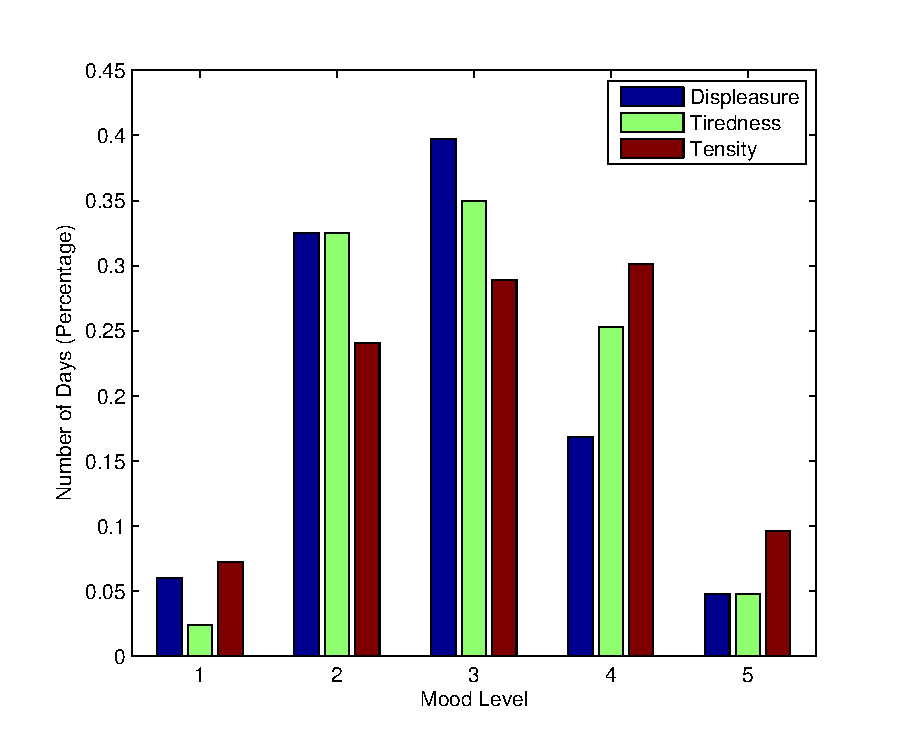
\includegraphics[width=15cm,height=10cm]{days}
  \caption{心境级别的分布}
  \label{mood:fig:mooddist}
\end{figure}

关于用户心境状态的时序分布方面,图\ref{mood:fig:moodcorr}展示了两个接连的时间槽(两天)内的心境状态差别分布。本图中,横轴表示这一时间槽与上一时间槽心境级别的差别(0代表没有差别)。从图中可以看出,每日的心境状态的时序关联关系非常显著,也即人们在连续的两天的心境状态通常是一致的,少有超过两个级别的非常极端的变化。这也验证了心境理论中的心境相对稳定性特征。
\begin{figure}[htbp]
  \centering
    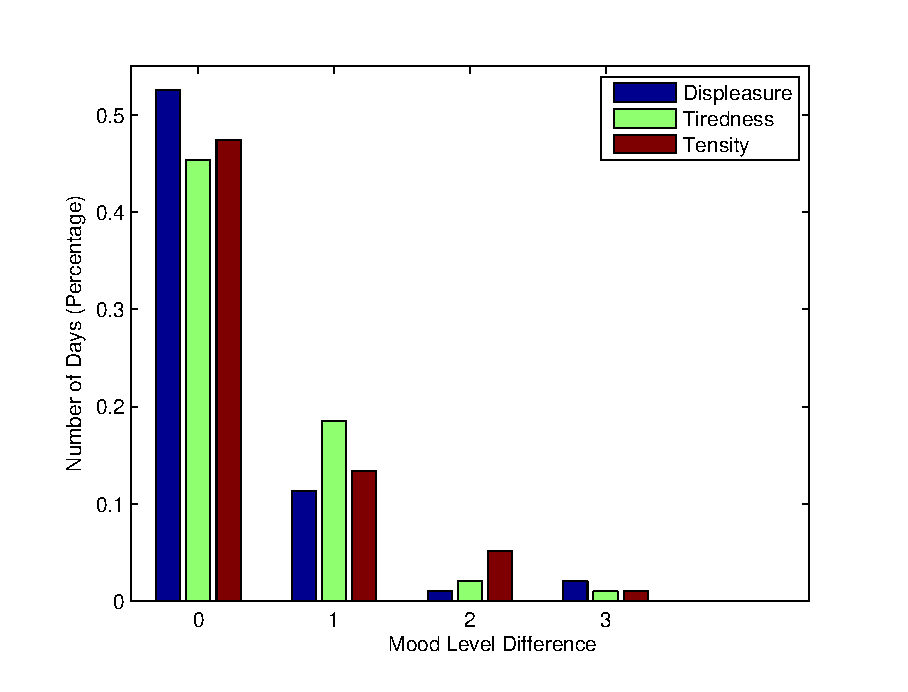
\includegraphics[width=15cm,height=10cm]{diff}
  \caption{连续两天内的心境差别分布}
  \label{mood:fig:moodcorr}
\end{figure}

在日常行为特征方面,我们分析了不同特征与心境状态之间的关联关系。作为示例,图\ref{mood:fig:minormotion}中展示了微动作与心境状态之间的关系。从图中可以看出,随着不愉快程度以及紧张程度的提高,微动作的数量也基本呈增加状态;而心境的活跃维度与微动作之间便没有显著的关联关系。从这可以看出,从传感器数据得到的日常行为特征与心境状态存在着关联关系,这也为使用贝叶斯方法利用手机感知的行为特征进行心境状态的评估提供了合理性。

\begin{figure}[htbp]
  \centering
    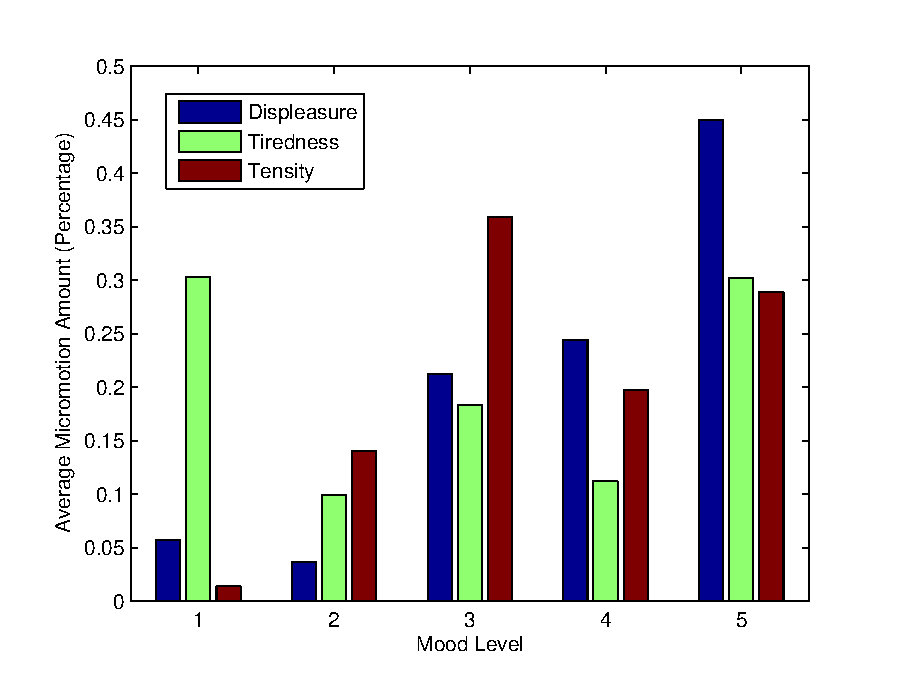
\includegraphics[width=15cm,height=10cm]{motion}
  \caption{不同心境状态下的微动作数量分布}
  \label{mood:fig:minormotion}
\end{figure}

\subsection{模型描述}
\label{mood:sec:ModelDescription}

基于对数据的观察结果,本文提出了一种基于因子图模型的分类算法,称为``社交-特征因子图''(Social-Featured Factor Graph,SFFG)。因子图模型是一个二元图模型,用以描述一类学习目标为包含多个变量的复杂全局函数的算法。这类算法中,全局目标函数被分解为多个``本地''函数的乘积,每个``本地函数''只包含全局函数的变量的一个较小的子集,并且函数形式更为简单\cite{factorgraph, followback}。

在详细描述模型之前,首先阐明几个基于实验数据观察的合理假设。首先,为简化模型,假设用户的心境状态具有马尔可夫性,也即用户上一时间槽内的心境状态只能影响紧接着的下一时间槽的心境状态,并通过对下一时间槽心境状态的影响来影响未来。这个性质可以如下表示:给定$m_i^{(t-1)}$,$m_i^{(t)}$与$m_i^{(t')}$对于所有$t' \leq t-2$条件独立。
我们也假设同一用户在同一时间槽内的不同行为特征关于此时间槽内的心境状态是条件独立的,也即给定$m_i^{(t)}$,所有$x_{ij}^{(t)} \in X_i^{(t)}$条件独立。 

基于上述的观察和假设,本文定义如下的因子函数:

\begin{itemize}
  \item \textbf{时序关联因子:} $tc(m_i^{(t-1)}, m_i^{(t)})$. 这个因子函数反映了心境的稳定性。基于前文提到的马尔可夫性假设,用户心境状态的衰减可以按如下函数建模:
  \begin{equation}
    tc(m_i^{(t)}, m_i^{(t-1)}) = exp\{-\lambda _i \| m_i^{(t)} -m_i^{(t-1)} \| \}
    \label{mood:tc}
  \end{equation}
  其中参数$\lambda_i$表示了用户\textit{i}的心境状态的时序衰减程度。  
  \item \textbf{特征关联因子:} $\textbf{c}(m_i^{(t)}, x_{ij}^{(t)})$. 每个用户行为特征$x_ij^{t}$都对用户$i$的心境$m_i^{(t)}$在不同维度上有不同程度的影响。本文使用朴素贝叶斯策略来建模特征的影响,用贝叶斯理论来建模$c(m_i^{(t)}, x_{ij}^{(t)})$,即先前观测到的取值组合具有更高的因子函数取值。

根据前文的假设,行为特征之间具有条件独立性,因此所有特征关联因子可以以如下的形式组合:
\begin{equation}
fe(m_i^{(t)}, \mathbf{x}_i^{(t)}) = \frac{1}{Z_\beta}exp\{\mathbf{\beta}^T\mathbf{c}(m_i^{(t)}) \mathbf{x}_i^{(t)}\}
\label{mood:fe}
\end{equation}
其中$\textbf{c}$代表特征关联因子向量,$\mathbf{\beta}$是一个权重向量,用来控制每个特征的相对权重,而$\frac{1}{Z_1}$为归一化因子。 

\item \textbf{社交关联因子:} $sc(m_i^{(t)}, m_j^{(t)})$. 社会关系的当前心境状态之间存在着相互影响。社交影响用如下函数建模:
\begin{equation}
sc(m_i^{(t)}, m_j^{(t)}) = exp\left\{ \alpha_i e_{ij}^{(t)} * (m_i^{(t)} -m_j^{(t)}) \right\}
\label{mood:sc}
\end{equation}
\end{itemize}
其中,$e_{ij}^{(t)}$为社交影响(参见定义\ref{mood:equ:e})。$\alpha_i$为权重参数,反应用户$i$的心境对于社会关系的易受影响程度。

最终,给定一个网络$G^{(t-1)} = \{\mathbf{V}, \textbf{E}^{(t-1)}, \mathbf{X}^{(t-1)}, \mathbf{m}^{(t-1)}\}$,以及当前的状态$\mathbf{X}^{(t)}$及$\mathbf{E}^{(t)}$,根据公式(\ref{mood:tc}),(\ref{mood:fe})与(\ref{mood:sc}),$M$上的联合概率分布为: 
\begin{equation}
\begin{split}
p(m|G^{(t-1)},& \mathbf{X}^{(t)}, \mathbf{E}^{(t)}) \\
=& \prod_i tc(m_i^{(t-1)}, m_i^{(t)})\,fe(m_i^{(t)}, \mathbf{x}_i^{(t)})\, sc(y_i^{t},H(y_i^{t-1})) \\
=& \frac{1}{Z} \prod_i exp \bigg\{-\lambda _1 \| m_i^{(t)} -m_i^{(t-1)} \|  \\
& + \mathbf{\beta}^T\mathbf{c}(m_i^{(t)}) \mathbf{x}_i^{(t)} + \sum_j \left(\alpha_i e_{ij}^{(t)} * (m_i^{(t)} -m_i^{(t-1)})\right) \bigg \}
\end{split}
\label{mood:target}
\end{equation}
其中$\mathbf{\lambda}$,$\mathbf{\beta}$及$\mathbf{\alpha}$为模型参数,$\frac{1}{Z}$为全局归一化因子。

SFFG的图形化表示见图\ref{mood:fig:sffg}。每个用户有其所有行为特征的取值以及心境状态,用户之间由社交影响因子$e$相连。输入的网络通过因子函数$tc$,$fe$以及$sc$生成全局概率分布

\begin{figure}[htbp]
  \centering
  \scalebox{0.75}{
    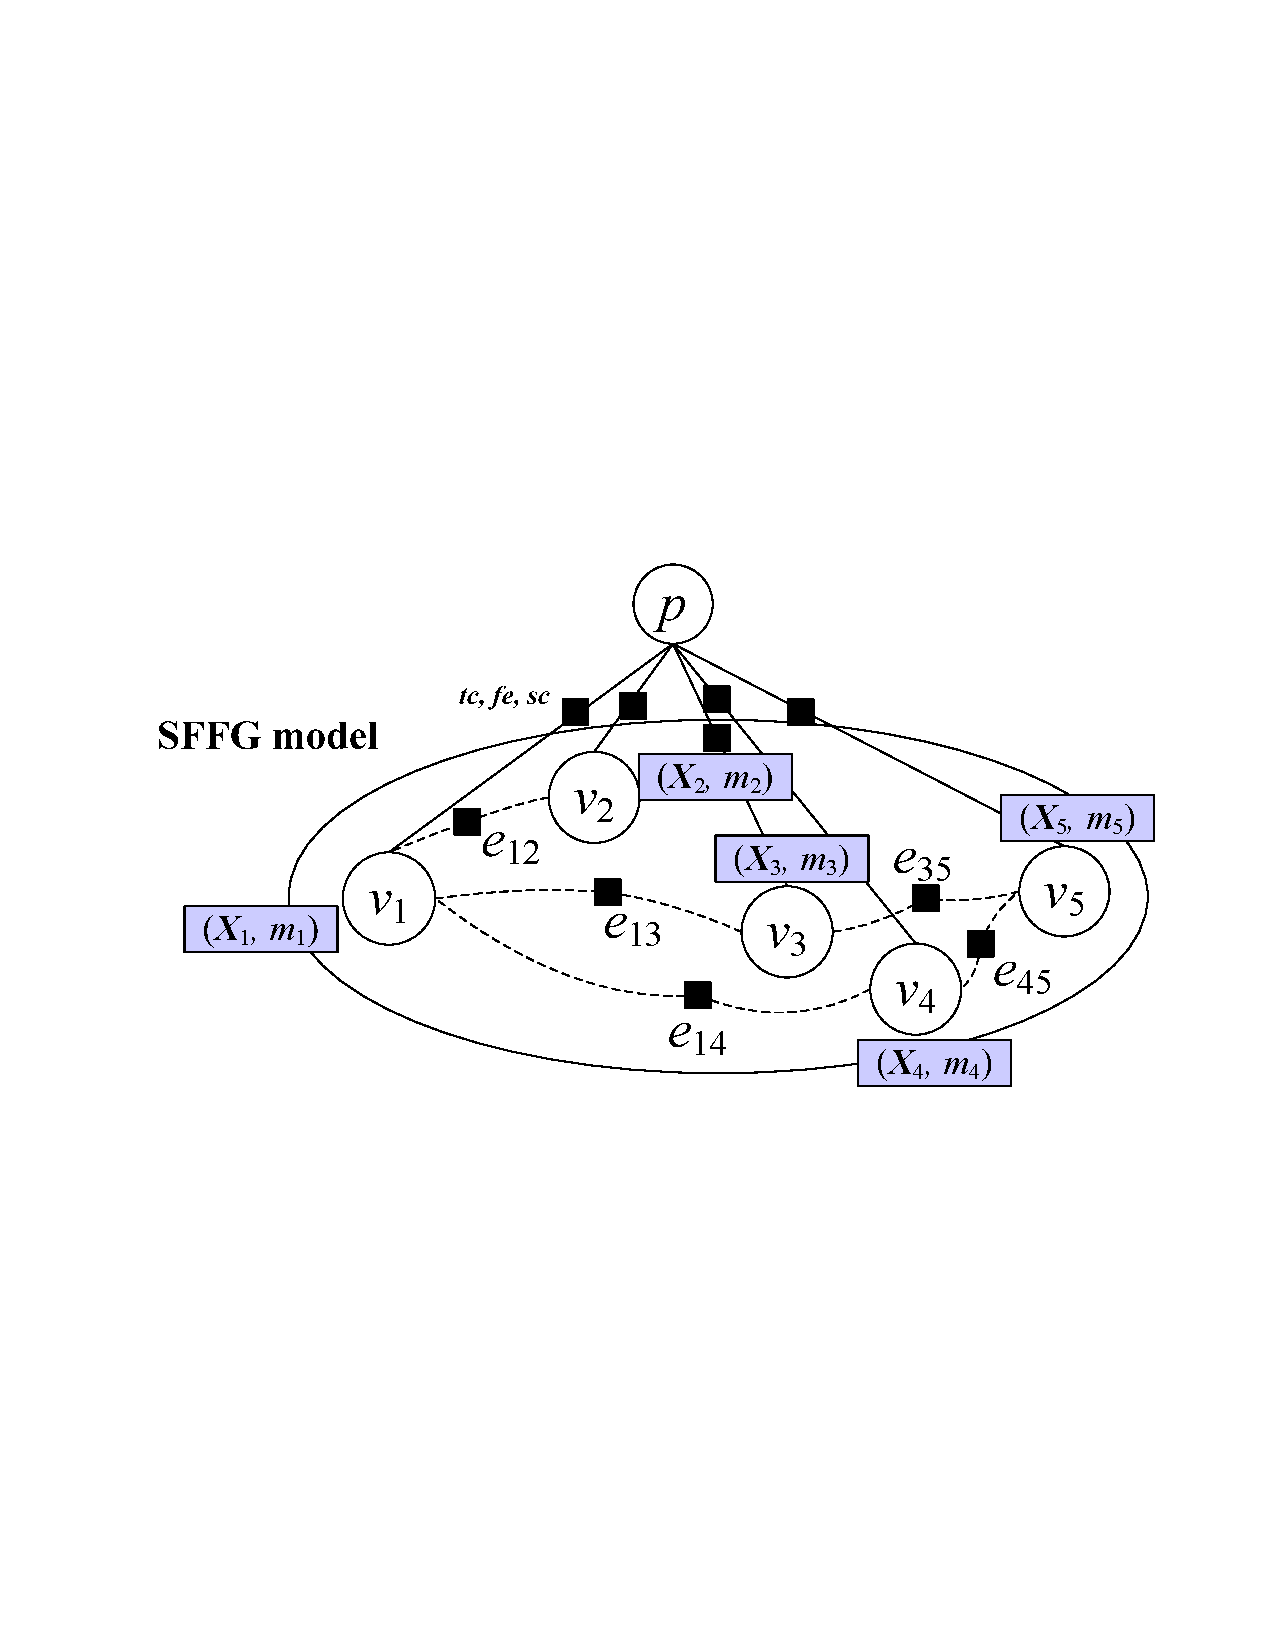
\includegraphics{sffg}
    }
  \caption{Visual depiction of SFFG model}
  \label{mood:fig:sffg}
\end{figure}


\subsection{SFFG模型学习}
\label{mood:sec:ModelLearning}
此模型的学习过程,也即训练参数$\theta = (\mathbf{\lambda}, \mathbf{\beta}, \mathbf{\alpha})$的最佳配置,以最大化给定训练数据上心境状态的对数似然:
\begin{equation}
\theta^* = {argmax}_\theta\left\{log\ p(\mathbf{m}|G^{(t-1)}, \mathbf{X}^{(t)}, \mathbf{E}^{(t)}, \theta)\right\}
\end{equation}
为了学习这样一个含有众多参数及全局归一化因子$Z$的目标函数,本文参与了基于Metropolis-Hastings (MH)抽样的算法。Metropolis-Hastings (MH)抽样算法为马尔可夫链蒙特卡洛方法(Markov-chain Monte Carlo,MCMC)的一个特例\cite{mh}\cite{socialEmotion}。

\begin{algorithm}
%\SetAlgoLined
\KwIn{learning rate $\eta$ which is the parameter that reflects the speed of learning}
\KwOut{optimal parameter $\theta = (\mathbf{\lambda}, \mathbf{\beta}, \mathbf{\alpha})$}

Initialize $\theta$;

\Repeat{Convergence}{
\% sample a new target variable configuration $\mathbf{m'}$
\[\mathbf{m'} \leftarrow q(\mathbf{m});\]
\[\tau \sim min(\frac{p(\mathbf{m'}|G^{(t-1)}, \mathbf{X}^{(t)}, \mathbf{E}^{(t)}, \theta)}{p(m|G^{(t-1)}, \mathbf{X}^{(t)}, \mathbf{E}^{(t)}, \theta)}, 1);
\]
%
\% generate a 0-1 random variable  $s$
\[s \sim Bernoulli(\tau, 1 - \tau);\]
%

\If{(s = 1)} 
{\
\% accept the new configuration $\mathbf{m'}$
\[ \mathbf{m} \leftarrow \mathbf{m'}; \]
\uIf{$(Err(\mathbf{m'}) < Err(\mathbf{m}) \Delta Ex|_\theta < 0) $}
{\[ \theta^{new} \leftarrow \theta^{old} + \eta(\Delta Ex|_\theta); \]}
\ElseIf{$(Err(\mathbf{m'}) > Err(\mathbf{m})  \Delta Ex|_\theta \geq 0) $}
{\[ \theta^{new} \leftarrow \theta^{old} - \eta(\Delta Ex|_\theta); \]}

}
}

\caption{模型学习算法}
\label{mood:alg:learning}
\end{algorithm}

MH算法分两个步骤。在第一步中,采用一个简单的抽样方法$q(\mathbf{m})$,从原目标配置$\mathbf{m}$中生成候选的新目标配置$\mathbf{m'}$。$q(\mathbf{m})$为简单地在目标配置空间全集$M$上按$m$的分布随机抽样。在第二步中,新的目标配置以概率$\tau$被接受:
\begin{equation}
\tau \sim min(\frac{p(\mathbf{m'}|G^{(t-1)}, \mathbf{X}^{(t)}, \mathbf{E}^{(t)}, \theta)}{p(m|G^{(t-1)}, \mathbf{X}^{(t)}, \mathbf{E}^{(t)}, \theta)}, 1)
\end{equation}

而后,如果新的配置$\mathbf{m'}$被接受,则更新模型参数$\theta$。参数的更新过程去觉得新旧配置$\mathbf{m}$与$\mathbf{m'}$的错误率$Err$,以及两个配置的对数似然差别$\Delta Ex|_\theta$: 
\[\Delta Ex|_\theta = Ex|_\theta (\mathbf{m'}) - Ex|_\theta(\mathbf{m})\] 
其中$Ex(\mathbf{m})$为公式\ref{mood:target}的指数部分($exp\{...\}$中包含的部分)

\section{算法评估}\label{mood:evaluation}


实验获取的数据集包含了2,872,311条手机传感器数据(包括加速度传感器,地理位置等),3,169条短信息记录,以及5,871条通话记录。 

收集到的原始数据按上文描述被聚合成特征,每个被试的每个特征每天有一个取值。
自报告的心境数据同样被聚合成每天一个取值(包含三个维度)。对于每天标注了多次心境状态的用户,取其所有标注值的加权平均值作为当天的心境状态,其中越晚的标注值权值越高。
被试用户被要求在每天的活动时间内在其手机上运行应用,并在夜间将要休息之前停止手机应用的数据采集,因为睡眠期间的传感数据并不能有效反应日常的行为,因此不能用来做每日心境评估。

由于此学习问题为针对离散的顺序级别的分类问题,本文采用准确度(预测的心境状态级别与报告的数据完全一致的人·天数占所有人·天数的比例),以及均方根误差(RMSE,root-mean-square error)作为模型表现的度量。模型的训练和测试采用了5份交叉验证的方法。

准确度的定义为: 
\[ accuracy = \frac{\sum_{u,d}{I_{(x_u^{(d)} = \widetilde{x}_u^{(d)})}}}{UD}
\]
均方跟误差的计算方法为:
\[
RMSE = \sqrt{\frac{\sum_{u,d}{{(x_u^{(d)} - \widetilde{x}_u^{(d)})}^2}}{UD}}
\]
其中$x_u^{(d)}$为评估结果,$\widetilde{x}_u^{(d)}$为实际的用户自报告值。$x$可以使三个心境维度$d$,$ti$或$te$中的任意一个。$I_s$ 为示性函数:当$s$为真时$I_s = 1$,反之$I_s = 0$。$U$和$D$为测试集中总的\textit{人·天}数。 


\begin{table}[htbp]
  \centering
  \caption{使用部分SFFG下MoodMiner的评估表现}
  \label{mood:tab:Performance}
    \begin{tabular}{|l|c|r|}
      \hline
      目标 & 准确度 & 均方根误差 \\
      \hline
      愉快度 & 52.58\% & 1.446 \\
      兴奋度 & 45.36\% & 1.519 \\
      放松度 & 47.42\% & 1.564 \\
      \hline
    \end{tabular}
\end{table}

\begin{table}[htbp]
  \centering
  \caption{使用完整SFFG下MoodMiner的评估表现}
  \label{mood:tab:Performance2}
    \begin{tabular}{|l|c|r|}
      \hline
      目标 & 准确度 & 均方根误差 \\
      \hline
      愉快度 & 71.68\% & 0.34 \\
      兴奋度 & 65.15\% & 0.361 \\
      放松度 & 65.60\% & 0.433 \\
      \hline
    \end{tabular}
\end{table}
使用SFFG评估模型,本文进行了两组模型实验。第一组实验中,只考虑了有时序因子及简单行为特征因子(包括地理位置,加速度,短信息频率,通话频率以及声音强度),模型的总体准确度稍低于50\%;第二组实验中,采用了完整的SFFG模型,包含了复杂的行为特征因子(活动姿态以及微动作),并且添加了社交影响因子。第二组实验的准确度提高了约20个百分点,达到了70\%左右。

\textbf{讨论.} 
评估模型的表现比较令人满意,最终达到了70\%左右的精度。最终输出的误差来源于多个方面。首先,由于心境天然的主观性,手机传感数据,通讯数据以及历史心境数据均有可能在一定情况下无法反映心境的波动 - 用户心境可能无任何征兆地突然变化。其次,人们在日常使用手机的模式上也存在很大的不同,使得统一的模型在不同用户身上可能出现较大的表现差别,很难让模型对于所有用户均有良好的表现。对于某些用户,功能强大的智能手机只有来接打电话和发信息,其余时间并不接触,使得本评估方法失败。另外,有些可能对心境评估产生作用的手机数据并未被采集,例如特定类型手机应用的使用情况;以及手机短信、电话功能外由应用提供的通讯方式(如\textit{Talkbox}\footnote{\url{http://talkboxapp.com/en/home}}及\textit{Skype}\footnote{\url{https://play.google.com/store/apps/details?id=com.skype.raider}}等)的使用情况
这些缺失的数据同样会影响模型最终的表现。


\section{本章小结}\label{mood:conclusion}

本章提出了一个单纯利用智能手机数据,通过用户行为分析来评估个人日常心境状态的新颖方法。首先定义了从手机数据中解析出的若干行为特征,而后提出了一个基于因子图模型的结合行为特征,时序关联和社交关联的心境评估方法。相较于传统的方法,这一方法具有用户干预少,客观,方便等优点,15个被试者延续了30天的实验表明,这一方法达到了令人满意的模型表现。
 

% % use section* for acknowledgement
% \section*{Acknowledgment}

% This work was supported in part by the National Science Foundation (NSF) of China, with grant No.61170212.

% % references section



% 如果要把编号的两个图形并排,那么小页就非常有用了:
% \begin{figure}
% \begin{minipage}{0.48\textwidth}
%   \centering
%   
\includegraphics[height=2cm]{thu-whole-logo}
%   \caption{并排第一个图}
%   \label{mood:fig:parallel1}
% \end{minipage}\hfill
% \begin{minipage}{0.48\textwidth}
%   \centering
%   
\includegraphics[height=2cm]{thu-whole-logo}
%   \caption{并排第二个图}
%   \label{mood:fig:parallel2}
% \end{minipage}
% \end{figure}

% 李氏子蟠,年十七,好古文、六艺,经传皆通习之,不拘於时,学於余。余嘉其能行古
% 道,作师说以贻之。

% \hfill \pozhehao 韩愈(唐)


\chapter{基于移动运营商数据的用户上网行为分析}
\label{cha:interest}

%%%\newdef{definition}{Definition}



\section{相关工作}
\label{interest:sec:relatedwork}

基于互联网使用记录的用户兴趣和行为挖掘长久以来便是一个热门的课题\cite{kdd00kosala}\cite{kdd00srivastava}\cite{widm01Mobasher}。 White等\cite{sigir09white}使用5种不同的上下文信息来建模用户兴趣,并依据用户兴趣进行推荐服务。Nasraoui等\cite{tkde08nasraoui} 通过追踪用户在某一特定网站的档案和行为,针对这一网站研究了用户的行为模式。也有些研究人员使用聚类方法来发现用户的类型\cite{icina10xu}\cite{kdex99mobasher}。然而,这些方法或者从用户的角度出发,将用户聚成不同的类型;或者从网站的角度出发,将网站URL聚合成不同的类型,而不是使用层次化多为聚类方法,在统一的模型中同时发现用户类型和网站类型。 

随着移动互联网在人们对互联网的总使用量中所占比重的不断增大,移动互联网中的用户行为也获得了研究者的关注\cite{pm2hw2n12almutairi}。Cui等\cite{www08cui}通过上下文获取方法,描述了人们在移动设备上使用互联网的方式,并分析了其中的上下文因素和用户行为模式。Tseng等\cite{ist06tseng}基于地理位置轨迹挖掘用户在移动互联网系统中的行为模式,并通过模拟实验进行了验证和分析。Phatak等\cite{fuzzy02phatak} 提出了基于距离矩阵的针对网站URL和用户的模糊聚类方法,并据此进行用户的建模和推荐服务。Do等\cite{mum10do}使用手机应用使用情况进行用户模式挖掘,其中包含了移动互联网使用记录。Verkasalo\cite{puc09verkasalo}手机了手持设备数据(包含移动互联网使用记录),从统计学角度分析了移动服务使用情况中的上下文模式。这些研究大多使用手机手机的数据,这些数据对于面向用户个体的行为分析可以胜任,但由于其难以规模化,限制了方法应用的规模和分析结果。本文提出的方法从移动运营商的角度,使用移动运营商的用户网络使用记录进行用户行为的分析与挖掘,保证了规模性型和全面性。

\section{数据描述}
\label{interest:sec:data}

本文使用的数据为某一移动运营商蜂窝网络(包括2G与3G)中的移动互联网使用记录(HTTP请求记录)。数据集覆盖的地理区域为北京市城区的一部分,集中在东城区和朝阳区的一部分,覆盖的区域面积约为40平方公里。区域内包含了故宫、天安门等热门景点,以及国贸、三里屯等重点商圈。区域内的常住居民约为90万。本数据集的时间跨度为2012年10月24日到2012年11月14日。

数据集中的每一条记录对应于一个发生在运营商蜂窝网络中的HTTP请求/响应对,数据的主要结构见表\ref{interest:tab:fields}。

\begin{table}
\centering
\caption{运营商数据集列结构}
\label{interest:tab:fields}
\begin{tabular}{|c|c|l|} \hline
名称 & 数据类型 & 描述\\ \hline
用户ID & 字符串 & 用户的唯一标识符\\ \hline
纬度 & 浮点数 & 移动基站的纬度\\ \hline
经度 & 浮点数 & 移动基站的经度\\ \hline
请求时间 & 时间 & 请求发生的时间\\ \hline
主机地址 & 字符串 & 被请求的主机的地址\\ \hline
内容类型 & 字符串 & HTTP协议中的ContentType域 \\
\hline\end{tabular}
\end{table}

\textbf{数据概览.} 数据集中包含的完整记录共有 \textbf{578,134,225} 条。对于数据的清理,采用了如下方法:
\begin{inparaenum}[\itshape 1\upshape)]
\item 数据分析关注于用户行为, 故使用\textit{内容类型}域将所有附加资源请求过滤掉(包括CSS,JavaScript以及附加图片等)。
\item 根据\textit{主机地址}域,将无意义的请求(如地址全是问号)过滤掉。
\end{inparaenum}
经过数据清洗之后,共有\textbf{66.823\% (386,332,325条)}的记录被保留下来。

\textbf{用户.} 数据集中出现过的独立用户数为\textbf{3,524,929}。图\ref{interest:fig:usertotalcountdist}中展示了用户的总请求数的分布情况。从图中可以看出,\textbf{40\%}的用户一周内发出的请求书少于10个;超过\textbf{95\%}的用户每周的请求书少于1,000个。每用户每周的平均请求数位\textbf{137.27}。

\begin{figure}
\centering
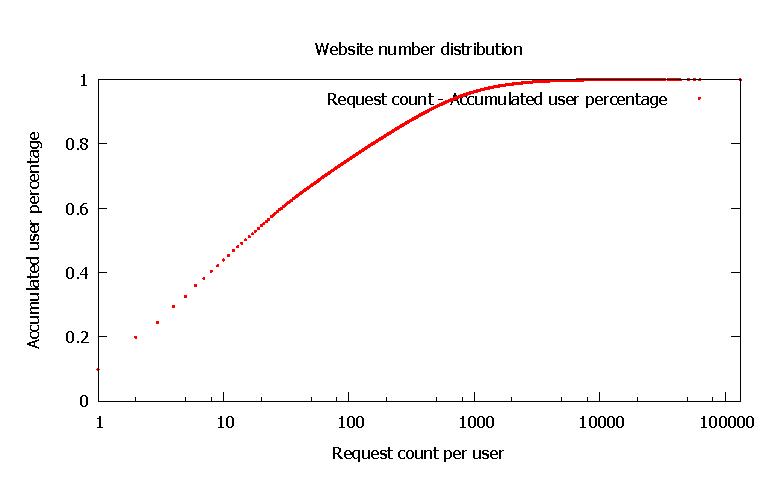
\includegraphics{user_conncount}
\caption{每用户请求数对应的用户数}
\label{interest:fig:usertotalcountdist}
\end{figure}

\textbf{主机地址.} 数据集中共出现了\textbf{363,841}个不同的主机地址。然而,只有\textbf{40.12\%}的主机地址被多于1个用户访问过。 按访问数降序排列,排名前990的主机地址占据了总记录数的97.877\%,而排名前10的主机地址占据了总记录数的58.1\%。可以看出,与传统桌面互联网相比,移动互联网中的网站/服务使用情况要集中得多。

\textbf{地理位置.} 数据集共涵盖了856个独立的蜂窝基站,每个基站由其经纬度唯一确定其位置。原始的基站数据对于用户行为建模来说意义不大,本文将基站聚类为地理区域后加入用户行为模型中。(详见第\ref{interest:sec:region}章)


\section{地理区域发现}
\label{interest:sec:region}
地理位置在移动互联网使用的上下文中占有重要的地位。用户所访问的网站与该访问行为发生的地点有着自然的联系,比如,相较于在住宅区的用户(通常在家里),CDB区域的用户更有可能通过手机使用本地搜索来查询附件的餐馆信息;与工作地点相比,人们更可能在家里使用手机阅读等等。
数据集中原始的地理位置信息(基站)力度太细,蕴含的语义信息太少。因此,在地理位置相关的挖掘中,通常把地点看成更大的地理实体的一部分,如地理区域\cite{env07park},或者轨迹\cite{www10zheng}\cite{debu10zheng}。在移动互联网使用的情境中,上网行为发生的所在地点的地理区域功能更为重要,本研究中,将位置点聚合成地理区域,后者作为用户行为模型中的因素考虑。
数据集中提供原始位置点(经纬度)为蜂窝基站的位置,基站覆盖范围(即位置精度)为50-150米。
\begin{definition}
\textbf{功能区域}. 城市的一个地理功能区域(以下简称为区域),定义为提供一个特定集合的城市功能的最小地理范围。某一区域所提供的功能集合对于绝大多数居民来说是一样的。
\end{definition}
如上定义的功能区域通常会包含数目不定的若干个基站,需要将基站聚类成区域,并且找出每个区域的功能特征。
\subsection{聚类算法}
本研究使用一个改进的DBSCAN算法来进行地理位置的聚类。

DBSCAN算法中的类簇定义基于密度可达性。算法中有两个参数:$\epsilon$和$MinPts$,通过这两个参数定义点的邻域($\epsilon-neighborhood$),从而判断密度可达性。下面介绍DBSCAN算法中的基本概念:

点$p$的$\epsilon-neighborhood$用$N_\epsilon(p)$来表示,定义为:$N_\epsilon (p)=\{q \in D|dist(p,q) \leq \epsilon \}$。对于聚类,直观的做法是,对于类簇中的所有点,该点的$\epsilon-neighborhood$中至少包含$MinPts$个点。
一个类簇是数据库中所有点集合的一个子集,其中包含的点满足两个属性:其中所有的点之家俩俩之间密度相连;如果某个点与类簇中的任意一个店密度相连,则其也属于这个类簇。\cite{ester1996density}

本文改变了$\epsilon-neighborhood$的计算方法。本研究中,$\epsilon-neighborhood$的定义中包含基于三种相似度/距离的限制规则:(A和B是两个基站)
\begin{itemize}
	\item 记录相似度$sim\_r$。$sim\_r$表示A和B在记录数量上的相似程度。处于同一区域内的基站,由于其功能的相似性,一天内不同时间段间记录数的分布情况也应具有较高的相似性。
	\item 迁移记录相似度$sim\_m$。如果用户$u$在A范围内有一条访问记录,短时间内在B范内又有一条访问记录,则称此为一次\textit{迁移记录}。迁移记录的多少体现了两个基站之间人员的流动成都,也体现了二者联系的紧密性。
	\item 地理距离$dg$。$dg_{(A,B)}$表示A与B之间的地理距离(单位为\textit{米})。
\end{itemize}
$sim\_r$的计算方法如下。考虑到用户访问行为在工作日和周末之间存在差别,因此对二者分别对待。以\textit{1小时}作为时间槽,共能得到48个关于一个基站的统计数据:工作日数据$vd_(A,i)$以及周末数据$ve_(A,i)$(i的取值范围是 0 到 23,代表24个小时)。$sim\_r_{(A,B)}$的计算见式\ref{interest:equ:simr}。
\begin{equation}
\label{interest:equ:simr}
	sim\_r_{(A,B)} = \frac{\sum_{i=0}^{23}{\left(\frac{vd_{(A,i)}}{vd_{(B,i)}} + \frac{ve_{(A,i)}}{ve_{(B,i)}}\right)}}{48}
\end{equation}

对于迁移记录相似度,A与B之间的总迁移记录数便能够反映二者之间联系的紧密性,不需要更细致的数据。用$m_{(A,B)}$来表示A与B之间的迁移记录总数,则$sim\_m$可按如下方法计算:

\begin{equation}
	sim\_m_{(A,B)} = \frac{m_{(A,B)}}{v_A}
\end{equation}
其中$v_A$为A基站内的所有记录总数。

值得注意的是,如此定义的相似度并不是对称的,也即$sim\_m_{(A,B)} \neq sim\_m_{(B,A)} $。在计算$\epsilon-neighborhood$的时候,双向的迁移记录相似度均被作为条件考虑。 

地理距离上的限制条件$dg$是可调整的。由于基站的密度在不同区域间存在很大差别,为此定义了两个级别的阈值$DG_s$与$DG_l$($DG_s < DG_l$),并且根据基站临近的其他基站数目来动态调整应用于$dg$的阈值。 

最终,综合三种距离/相似度上的限制来确定某一基站的$\epsilon-neighborhood$,详见算法\ref{interest:alg:neighber}。
如果计算得到的A基站的$\epsilon-neighborhood$不为空,则将A视为DBSCAN中的核心点
\begin{algorithm}
%\SetAlgoLined
% \KwIn{基站A;\\ 
% 所有基站的集合$\mathbf{C}$;\\
% 阈值的默认取值$SIM\_R_0$,$SIM\_M_0$,$DG_s$以及$DG_l$;
% 参数$MinPts$}
% \KwOut{${\epsilon-n}_A$,即基站A的$\epsilon-neighborhood$内的所有基站}

% 初始化 ${\epsilon-n}_A$ 为空集;
\KwIn{Cellular tower A;\\ 
Set of cellular towers $\mathbf{C}$;\\
Default values of thresholds $SIM\_R_0$, $SIM\_M_0$, $DG_s$ and $DG_l$;
Value of parameter $MinPts$}
\KwOut{${\epsilon-n}_A$, containing all other cellulars in the $\epsilon-neighborhood$ of A}

Initialize ${\epsilon-n}_A$ as empty set;

Initialize thresholds $SIM\_R \leftarrow SIM\_R_0$, $SIM_M \leftarrow SIM\_M_0$, $DG \leftarrow DG_s$

\For{Each other cellular $B \in \mathbf{C}$}{
		\If{A and B are neighbors under current threshold configuration}{
			Add B to ${\epsilon-n}_A$;
		} 
}
\If{${\epsilon-n}_A$ is empty \textbf{and} $DG = DG_s$}{
		$DG \leftarrow DG_l$;
		
		Restart the For loop
}
\If{Size of ${\epsilon-n}_A \geq MinPts$}{
	Add A to ${\epsilon-n}_A$;
} \Else {
	Reset ${\epsilon-n}_A$ to empty;
}
Return ${\epsilon-n}_A$;
\caption{计算某一基站的$\epsilon-neighborhood$}
\label{interest:alg:neighber}
\end{algorithm}

\begin{algorithm}
%\SetAlgoLined
\KwIn{Cellular tower A and B (A $\neq$ B); 

Values of thresholds $SIM\_R$, $SIM\_M$, and $DG$}
\KwOut{Whether B is in the $\epsilon-neighborhood$ of A}
	\If{$dg_{(A,B)} > DG $}{
		Return FALSE;
	}\Else{
		Compute $sim\_r_{(A,B)}$ and $sim\_m_{(A,B)}$;
		
		\If{$1 < sim\_r_{(A,B)} \leq SIM\_R$ \textbf{or} $1 < sim\_r_{(B,A)} \leq SIM\_R$}{
			Return TRUE;
		}\ElseIf{$1 < sim\_m_{(A,B)} \leq SIM\_M$ \textbf{or} $1 < sim\_m_{(B,A)} \leq SIM\_M$}{
			Return TRUE;
		}
	}

\caption{判断两个基站是否临近(密度可达)的算法}
\label{interest:alg:pair}
\end{algorithm}

\subsection{聚类结果}
使用上述算法和参数配置,717个基站被聚类成126个区域,剩余的139个基站为单基站区域,总计得到265个区域。所得区域在地图上的分布见图\ref{interest:fig:regions}。

\begin{figure}
\centering
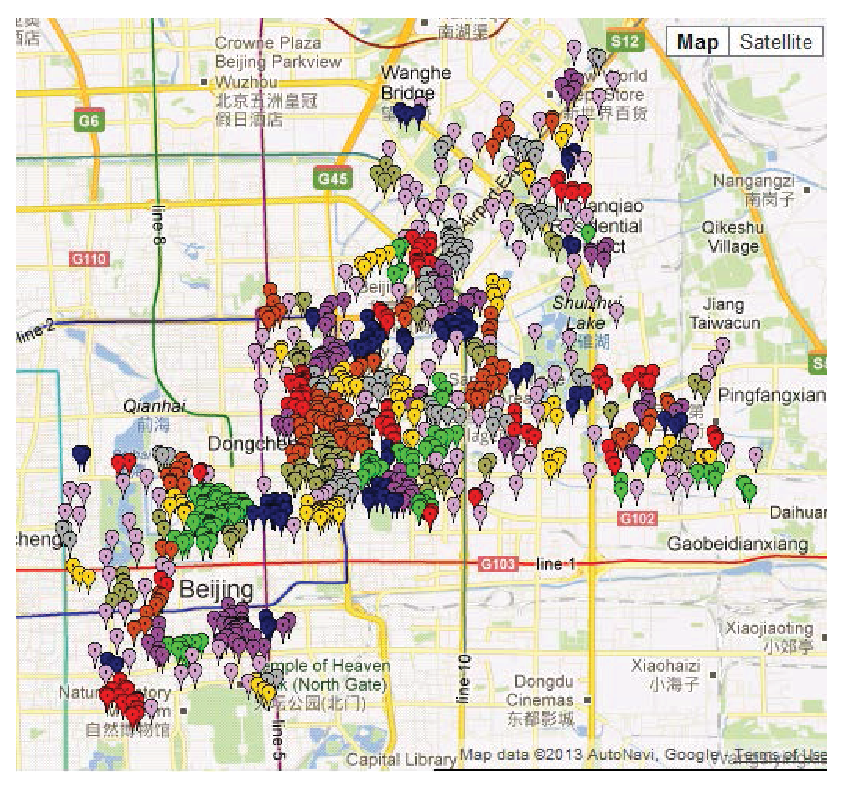
\includegraphics{regions}
\caption{以区域内基站标识的区域分布图}
\label{interest:fig:regions}
\end{figure}

为评估算法的分类结果,实验中试用了手工标注的每个基站所属的区域功能类型(数据来源于移动运营商)。
区域类型被进一步分成5个类别:\textit{居住区,工作区,活动区,学校}以及\textit{其他}。使用这些数据来分析126个聚类所得区域的准确性。

每个聚类所得区域被赋予一个分数。首先,将本区域内出现频率最高的类型作为本区域的功能类型。而后计算本区域内属于此类型的基站所占的比例$p$。
如果$p \geq 0.5$,表示此区域半数以上的基站具有同样的功能类型,那么这个区域的分数则为$p$。反之,如果$p < 0.5$,则认为这个区域的聚类不合理,其分数为0。

最终,126个区域中有99个区域的分数大于0.5,所有区域的平均得分为0.66。

以故宫周围区域为例进行说明(见图\ref{interest:fig:fob}):可以看到,故宫内的基站和王府井地区的基站被成功的分到了不同的区域内。然而,故宫内的基站也被分成了两个区域:北侧和南侧。这是因为故宫中央的基站过于稀疏,无法将南北两个区域连接起来。

\begin{figure}
\centering
\scalebox{0.75}{
	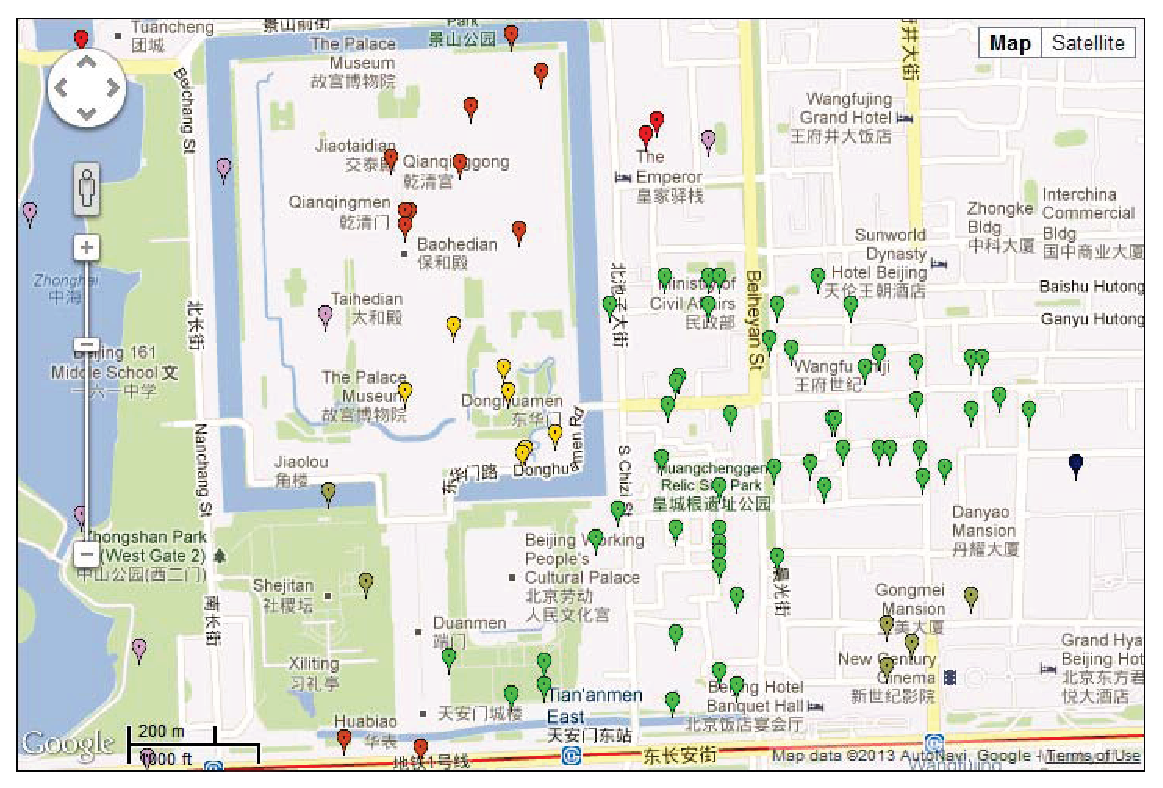
\includegraphics{forbidden}
}
\caption{故宫附近的区域分布情况}
\label{interest:fig:fob}
\end{figure}

针对27个``不合理''区域进行分析,人工检查其中的基站发现,其中的绝大部分基站的类别标识为``高密度居民区''以及``企业办公区'',可以推断这些地区包含综合功能大厦,低层用于商业活动,高层作为居住区。按照前文对于区域的定义,这些区域也是符合要求的混合功能区域,在模型中可以作为一个整体对待。故总的来说,聚类结果对于建模需求来说是可靠的。


\section{用户兴趣发现模型}
\label{interest:sec:uri}
首先给出``用户兴趣''的定义。

\begin{definition}
\label{interest:def:ui}
\textbf{用户兴趣}. 某个户的兴趣表示该用户感兴趣、喜欢浏览或使用的某一特定类型的网站或服务。一个用户可能有多种不同的兴趣,每个兴趣有一个权值,代表该用户对这个兴趣的喜爱程度。另一方面,用户兴趣也可能表示网站或服务的风格而不是类型,一个网站也可能属于多种不同的用户兴趣类型。
\end{definition}

为了从移动互联网使用记录中抽取隐含的用户兴趣,,本文提出了一个基于LDA(Latent Dirichlet Allocation)的概率话题模型方法。在这个模型中,抽取出来的隐含层即表示定义\ref{interest:def:ui}中的\textit{用户兴趣}。

话题模型是目前在文本挖掘中常用的建模方法,用以发现一个文档集中隐含的``话题''层。LDA(Latent Dirichlet Allocation)\cite{jmlr03blei}是一个目前最常用的话题模型,而且被扩展应用于除了词之外的其他文档属性(作者,会议,等等)\cite{kdd04steyvers}\cite{kdd08tang}\cite{kdd12tang}。也有研究者将LDA及其扩展模型应用于用户行为模式的发现\cite{tist11farrahi}。LDA是一个非监督的生成模型,将一篇文档的生成过程(每个词的撰写过程)分成两个阶段:第一阶段为根据文档上的话题分布选择一个话题;第二阶段为根据话题上的次分布选择一个词。

使用访问的网站集合来表示用户,类似LDA中的文档,而后对其进行话题模型建模。

\subsection{网站发现}
\label{interest:sec:website}
本章将介绍从原始的移动互联网HTTP访问记录抽取网站的方法。

首先,给出一些模型中常用概念的定义。

\begin{definition}
\textbf{用户}:用户在数据集中由\textit{用户ID}唯一标识,并唯一对应于一个使用移动互联网的自然人(一个手机号码),无论其使用的是否为同一个联网设备。
\end{definition}

\begin{definition}
\label{interest:def:host}
\textbf{主机}:主机即HTTP请求中的被请求主机,由主机地址(URL)唯一确定。此地址可能是,也可能不是用户/应用直接访问的地址。
\end{definition}

根据常识以及对数据的观察,第三级及以上的域名(如果此主机地址的顶级域名为国家/地区域名,二级域名为通用域名,如\textit{.com.cn},则是第四级及以上的域名)在标识不同的网站/服务上并不起作用。\footnote{如QQ,Baidu等超大型移动互联网服务公司的域名除外,它们下属的子域名可能会提供完全不同的服务。这种情况下多加一级的域名会被保留下来。}基于上述观察,原始数据经过一次预处理,将URL中不起作用的部分移除,保留下来的部分作为主机地址唯一标识主机。实验表明,没有这一步预处理的情况下,来自同一根域名的不同地址会在话题模型中形成干扰。

网站与被地址唯一标识的主机并不完全等同(参见定义\ref{interest:def:host})。当用户访问某一网站时,可能会对不同的主机地址发出多个请求。因此,需要首先将主机聚类,每个类代表一个网站。

\begin{definition}
\textbf{网站}. 一个网站代表一个给用户提供内容或服务的独立主体,可能使用多个不同的主机地址。 
\end{definition}

网站和主机并没有很强的关联关系。例如,网站\textit{qq.com}是一个腾讯旗下的知名门户网站,而其子域名\textit{t.qq.com}则是腾讯旗下的微博网站,二者并不属于同一网站;另一方面,\textit{t.sina.com.cn}和\textit{weibo.com}主机地址完全不同,但都是新浪微博的地址,所以按照上述定义,他们应属于同一网站。

将主机聚类成网站的算法描述如下。首先,将每个主机看成一个向量$H_i: <C_{h_i, u_1}, C_{h_i, u_2},...,C_{h_i, u_n}>$,其中$C_{h_i, u_j}$是用户$j$向主机$i$发出的请求数。而后,使用这一向量表示计算主机俩俩之间的余弦相似度。之后设定一个阈值$\alpha$,将所有相似度高于$\alpha$的主机对儿看成同一网站内的主机。

实验中,使用了从0.1到0.9范围内的不同$\alpha$值,不同阈值与所得的网站数量的对应关系见图\ref{interest:fig:websitecount}。由于在用户行为模型中,网站被视为一种最小单元,故在网站发现的过程中,应更关心聚类的准确度,所以倾向于选择更大的$\alpha$值。 基于图中曲线的形状,以及对聚类结果的观察,最终选定的$\alpha$值为\textbf{0.5}。在此阈值下,生成的网站示例如:``Website No.580: wikipedia.org, wikimedia.org'',``Website No.357: adsmogo.mobi, adsmogo.org, adsmogo.com''。

使用\textbf{0.5}作为阈值共得到924个网站。其中大部分的网站仍然只包含一个主机,最大的一个聚类包含5个主机。

\begin{figure}
\centering
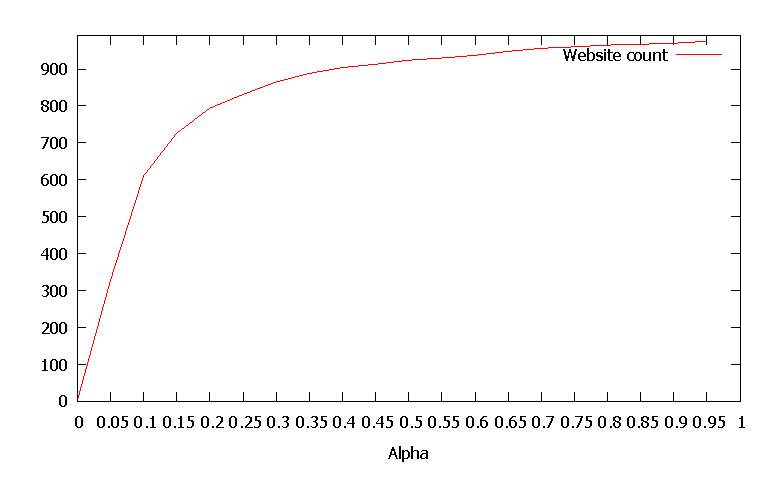
\includegraphics{alpha_websitecount}
\caption{网站数量与聚类阈值的关系图}
\label{interest:fig:websitecount}
\end{figure}

\subsection{用户的网站向量表示} 

模型中将用户视为文档,将网站视为词。网站在用户表示中的每一次出现(即该用户访问了该网站)都被关联以一个区域,对应与该次访问行为所发生的区域。

由于原始的HTTP记录并不能忠实地反映用户的行为,在生成表征用户的向量时,对原始记录进行了转换处理。处理过程如下:
首先,将一天分成48个半小时跨度的时间槽,并将每个时间槽作为表示用户行为的稳定时间段(即半小时内用户的网站访问行为基本稳定)\cite{tist11farrahi}。而后,对于每个用户$u$以及每个时间槽$t$,排名前三的访问量最大的网站被视为在这个时间槽内被该用户``访问''。对于每个被访问的网站$w$,用户$u$在时间槽$t$内访问$w$的所有记录中出现次数最多的区域被视为关联到这次$w$的访问的区域。于是,一个用户可以被如下表示:$U = \{{<w_{ui}, r_{ui}, c_{u,w_{ui},r_{ui}}>}\}$,其中$c_{u,w_{ui},r_{ui}}$是用户$u$访问$<w_{ui}, r_{ui}>$的次数。

\subsection{用户-区域-兴趣(URI,User-Region-Interest)模型}
本文将用户,网站,地理区域,以及用户兴趣综合考虑,用同一的生成模型进行建模。按对``用户兴趣''这一隐含层的实际解释不同,以及在生成过程中考虑\textit{区域}的策略的不同,提出了两种不同的生成过程,以及对应的两种不同的URI模型。

\textbf{URI1模型} 在第一个模型(URI1)中,隐含的``用户兴趣''层被视为用户频繁的网络使用模式,与用户一方的联系更为紧密。每个用户有一个``用户兴趣''的分布,这一份不与地理位置无关;同时,每个``用户兴趣''中,针对每个区域有一个不同的网站分布。这一模型下的生成过程如下(见图\ref{interest:fig:uri}):
\begin{enumerate}
	\item 对于每个用户$u$,根据狄利克雷先验$\alpha$生成$\theta_u$;
	\item 对于每个用户兴趣$z$, 根据狄利克雷先验$\beta_z$,对每个区域$r \in R$生成$\phi_{(z,r)}$;
	\item 对于用户$u$内的每此网站访问$w_{ui}$:
	\begin{itemize}
		\item 根据多项分布$theta_u$生成$z_{ui}$;
		\item 根据多项分布$\phi_(z_{ui},r_{ui})$生成网站$w_{ui}$。
	\end{itemize}
\end{enumerate}

模型的参数估计部分使用吉布斯抽样(Gibbs sampling)方法\cite{nas04griffiths}。简单化考虑,对超参数取值$\alpha$和$\beta$采取了固定取值(如,$\alpha = 50 / T$, $\beta = 0.01$)。使用吉布斯抽样方法来估计$w$,$z$以及$r$的后验概率分布,而后用结果来估计$\mathbf{\theta}$以及$\mathbf{\phi}$。
后验概率的计算方法是:
	\begin{equation}
	P(z_{ui}|\mathbf{z_{-ui}},\mathbf{w}, \mathbf{r}, \alpha, \beta) \propto
	  \frac{m^{-ui}_{u,z_{ui}} + \alpha_{z_{ui}}}{\sum_{z}{(m^{-ui}_{u,z} + \alpha_z)}}
		\frac{n^{-ui}_{z_{ui},r_{ui},w_{ui}} + \beta_{w_{ui}}}{\sum_{w}{(n^{-ui}_{z_{ui},r_{ui},w} + \beta_w)}}
\end{equation}
其中$m_{u,z}$表示在吉布斯抽样中,兴趣$z$被分配给用户$u$的次数,$n_{z,r,w}$表示兴趣$z$在区域$r$内被分配给用户$w$的次数。上标$-ui$表示此技术并不包含当前的实例。

抽样过程收敛后,多项分布参数$\theta$和$\phi$使用如下方法计算:

\begin{equation}
	\theta_{u,z} = \frac{m_{u,z} + \alpha_z}{\sum_{z'}{(m_{u,z'} + \alpha_{z'})}}
\end{equation}
\begin{equation}
\label{interest:equ:phi}
	\phi_{z,r,w} = \frac{n_{z,r,w} + \beta_w}{\sum_{w'}{(n_{z,r,w'} + \beta_{w'})}}
\end{equation}

\begin{figure}
\centering
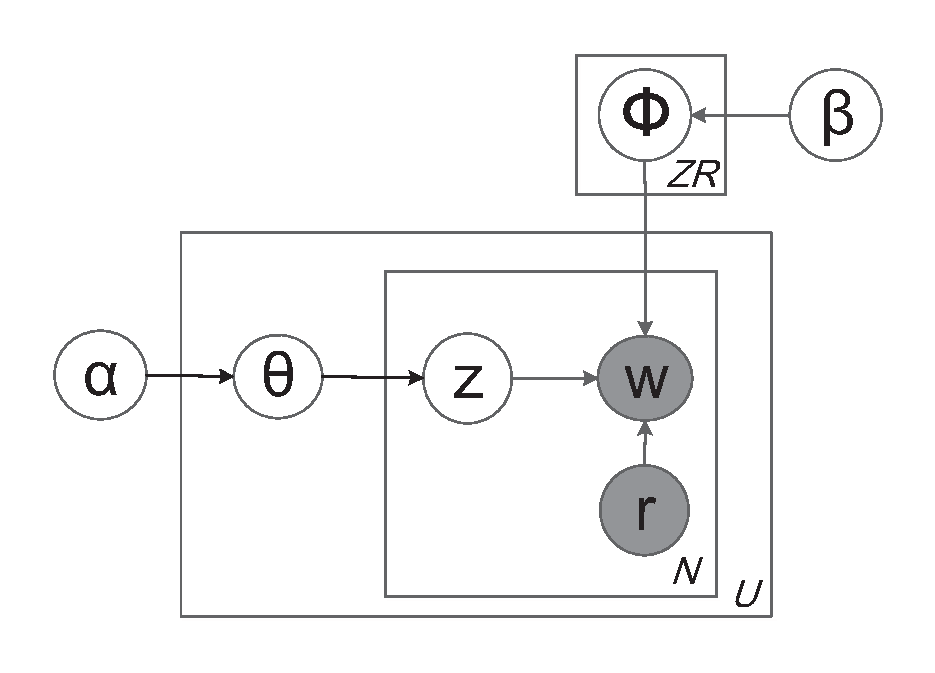
\includegraphics{uri}
\caption{User-Region-Interest (URI) 模型1 的盒图表示}
\label{interest:fig:uri}
\end{figure}

\textbf{URI2模型} 在第二个模型(URI2)中,隐含的``用户兴趣''层被看成是常见的经常同现的网站集合,与网站的联系更为紧密。每个``用户兴趣''上有一个所有网站的分布,这一分布与地理位置无关;而每个用户上的``兴趣''分布则与地理位置有关。URI2的生成过程如下(见图\ref{interest:fig:uri2}):
\begin{enumerate}
	\item 对于每个用户$u$, 根据狄利克雷先验$\alpha_u$,对每个区域$r \in R$生成$\theta_{(u,r)}$;
	\item 对于每个用户兴趣$z$, 根据狄利克雷先验$\beta$生成$\phi_z$;
	\item 对于用户$u$内的每此网站访问$w_{ui}$:
	\begin{itemize}
		\item 根据多项分布$theta_{(u,r_{ui})}$生成$z_{ui}$;
		\item 根据多项分布 $\phi_{z_{ui}}$生成网站$w_{ui}$。
	\end{itemize}
\end{enumerate}

与URI1模型类似,使用吉布斯抽样方法来估计模型参数。超参数同样被设定为固定值(如$\alpha = 50 / T$,$\beta = 0.01$),后验概率的计算方法为:
	\begin{equation}
	P(z_{ui}|\mathbf{z_{-ui}},\mathbf{w}, \mathbf{r}, \mathbf{\alpha}, \mathbf{\beta}) \propto
	  \frac{m^{-ui}_{u,r_{ui},z_{ui}} + \alpha_{z_{ui}}}{\sum_{z}{(m^{-ui}_{u,r_{ui},z} + \alpha_z)}}
		\frac{n^{-ui}_{z_{ui},w_{ui}} + \beta_{w_{ui}}}{\sum_{w}{(n^{-ui}_{z_{ui},w} + \beta_w)}}
\end{equation}

$\theta$和$\phi$的估计方法为:

\begin{equation}
\label{interest:equ:theta2}
	\theta_{u,r,z} = \frac{m_{u,r,z} + \alpha_z}{\sum_{z'}{(m_{u,r,z'} + \alpha_{z'})}}
\end{equation}
\begin{equation}
	\phi_{z,w} = \frac{n_{z,w} + \beta_w}{\sum_{w'}{(n_{z,w'} + \beta_{w'})}}
\end{equation}

\begin{figure}
\centering
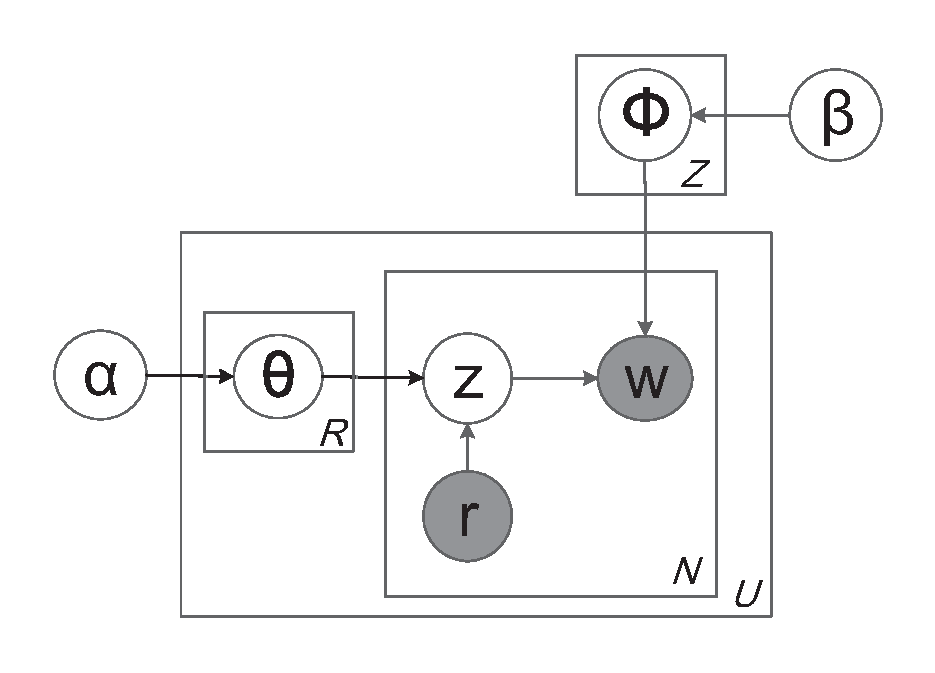
\includegraphics{uri2}
\caption{User-Region-Interest (URI) 模型2 和盒图表示}
\label{interest:fig:uri2}
\end{figure}


\section{实验}
\label{interest:sec:exp}

本章将展示在数据集上应用模型的结果,并给予实验结果进行分析讨论。
\subsection{实验数据}
\label{interest:sec:expdata}
实验使用的数据描述见第\ref{interest:sec:data}章。首先,实验选取了访问量前990的网站,它们只占网站总数的0.27\%,却占据的总访问量的97.877\%。此后,对于数据集中出现的所有用户,按照前文描述生成器网站向量表示。对于生成的用户集合,将其中包含5个以上不同的网站-区域对的用户是为活跃用户。将不活跃用户过滤掉以后,保留的活跃用户数为\textit{469,297},占原用户总数(\textit{3,524,929})的13.31\%。在所有的\textit{386,332,325}记录中,经过两步过滤,\textit{263392870 (68.18\%)}条记录保留了下来。

每个时间槽内的活跃用户数见图\ref{interest:fig:usercount}。从图中可以看出,在经过表示形式转换之后,曲线能够很好的和现实生活中的生活模式相匹配。

\begin{figure}
\centering
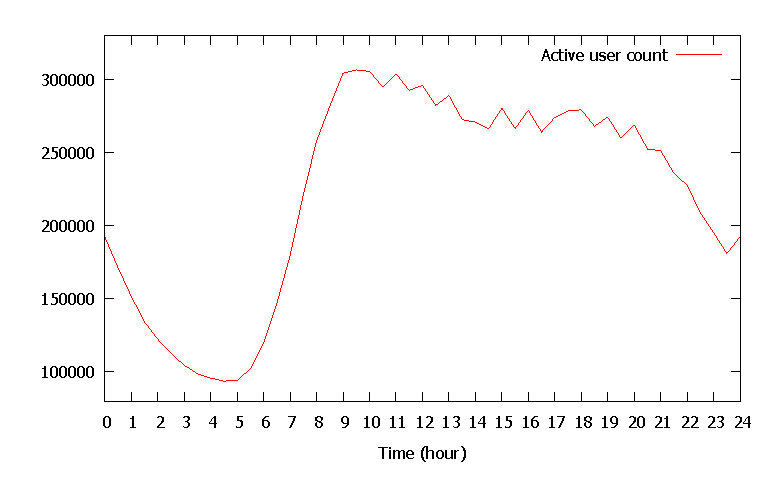
\includegraphics{user_timeslot}
\caption{Active user count over time}
\label{interest:fig:usercount}
\end{figure}

实验中使用不同的抽样方法生成了多个子数据集供训练和测试。除了完整数据集之外,通过随机抽样得到了两个子地理区域,各包含50,000个用户,完整数据集和两个随机抽样数据集分别用$d0$,$d1$及$d2$表示。除了按地理位置随机抽样以外,还将记录按时间来分割,给每个数据集生成了两个子集,分别包含前十天和后十天的记录。每个数据集的两个子集以后缀$-f$和$-l$来分别标识。

\subsection{用户兴趣发现}
实验中使用用户数$U = 469,297$,网站数$W = 924$,以及区域数$R = 265$来进行模型评估。实验中分别在同样的数据集上应用了两种URI模型以及传统LDA模型(使用传统的LDA生成过程)。为了比较,在LDA的抽样过程了,同样记录了每个词所对应的地理区域,而后使用式\ref{interest:equ:phi}来计算一个$K \times R \times W$的$\Phi$的参数矩阵,并使用式\ref{interest:equ:theta2}来计算一个$M \times R \times K$的$\Theta$的参数矩阵,其中$M$为训练集中的用户数。此处,原始的LDA中的$\Phi$和$\Theta$被称为$\Phi0$和$\Theta0$。同时称使用$\Phi0$和$\Theta0$的LDA模型为LDA0,使用$\Phi$和$\Theta0$的模型为LDA1,使用$\Phi0$和$\Theta$的模型为LDA2。
%We also calculated $\Phi0$ for URI model, using the same formula as in LDA:
%\begin{equation}
%	\phi0_{z,w} = \frac{n_{z,*,w} + \beta_w}{\sum_{w'}{(n_{z,*,w'} + \beta_{w'})}}
%\end{equation}
%where $n_{z,\bullet,w}$ means the sum of $n_{z,r,w}$ for each $r \in \mathbf{R}$.

\textbf{评价指标.} 实验中使用``用户兴趣''间的平均Jensen–Shannon差异来评估生成的隐含``兴趣''层的质量。Jensen–Shannon差异(JSD)是评价描述同一随机变量的概率分布间的相似度的常用方法。使用不同的$\Phi$和$\Theta$矩阵作为参数,就能够算出每个模型的JSD。
对于LDA1模型和URI1模型,每个``用户兴趣''内的网站分布于区域有关,JSD的计算方法是:
\begin{equation}
	JSD = \frac{\sum^T_{i=0}\sum^T_{j=i+1}\sum^R_{r=1}{jsd(\mathbf{\phi_{i,r}}, \mathbf{\phi_{j,r}})}}{\frac{T(T+1)}{2} \times R}
\end{equation}
对于其余的模型(LDA0,LDA2以及URI2),JSD的计算方法是:
\begin{equation}
	JSD = \frac{\sum^T_{i=0}\sum^T_{j=i+1}{jsd(\mathbf{\phi0_{i}}, \mathbf{\phi0_{j}})}}{\frac{T(T+1)}{2}}
\end{equation}


为评估模型重现真实的用户行为的能力,实验使用前10天范围内的数据(后缀为\textit{-f}的数据子集)来进行模型训练,而后使用同一数据集的另一数据子集(后缀为\textit{-l})来进行测试(关于数据集的描述参见第\ref{interest:sec:expdata}章)。

所有上述描述的模型均用于估计用户在测试集中的网站访问情况。
使用$d-f$表示训练集,$d-l$来表示测试机,用户$u$在数据集$d-l$中的实际网站分布为:
\begin{equation}
	\widetilde{pl}_{u,w} = \frac{cl_{(u,w,\bullet})}{cl_{(u,\bullet,\bullet)}}
\end{equation}
其中$cl_{u,w,r}$表示数据集$d-l$中,网站$w$在区域$r$内被用户$u$访问的情况($\bullet$表示$所有$)。 

将地理位置信息视为用户的上下文,每个用户的实际地理位置分布为:

\begin{equation}
	\widetilde{ql}_{u,r} = \frac{cl_{u,\bullet,r}}{cl_{u,\bullet,\bullet}}
\end{equation}
 
使用$\Theta$和$\Phi$,能够得到模型输出的估计的分布:
对于LDA1模型和URI1模型:
\[
	p_{u,w} = \sum_i{\left(\theta_{u,i}  \sum_r{(\phi_{i,r,w} \times ql_{u,r})}\right)}
\]
对于LDA2和URI2模型:
\[
	p_{u,w} = \sum_r{\left(\sum_i{\theta_{u,r,i} \times \phi_{i,w}} \times ql_{u,r})\right)}
\]
对于传统LDA模型(不考虑地理位置信息):
\[
	p_{u,w} = \sum_i{(\theta_{u,i} \times \phi_{i,w})}
\]

%For comparison, we also use the distribution of user $u$ on the complete dataset (containing both \textit{-f} and \textit{-l}) to infer $\widetilde{pl}_{u,r}$. In this case, the estimated distributions (with and without considering location) can be calculated as:
%\begin{equation}
%	p_{u,w} = \sum_r{\left(\frac{c_{(u,w,r)}}{c_{(u,\bullet,r)}} \times \widetilde{ql}_{u,r}\right)}
%\end{equation}
%\begin{equation}
%	p0_{u,w} = \frac{c_{(u,w,\bullet)}}{c_{(u,\bullet,\bullet)}}
%\end{equation}
%where $c_{(u,w,r)}$ means the same as $cl_{(u,w,r)}$, except in the complete dataset.

估计得到的用户的网站分布可以看成是他们对于网站的(潜在)偏好,这些信息可被用来理解用户行为模式,也可以用来进行推荐。实验中使用混乱度(perplexity)来评估这些模型生成的概率分布的表现。Perplexity是评估一个估计的概率分布还原真实分布(预测真实分布的样本)能力的常用度量方法。其定义为:
\[
perp(\mathbf{\widetilde{p}},\mathbf{q}) = 2^{H(\mathbf{\widetilde{p}},\mathbf{q})},
\]
其中指数$H(\widetilde{p},q)$为交互熵:
\[
H(\mathbf{\widetilde{p}},\mathbf{q}) = - \sum_x{\widetilde{p}(x)log_2^{q(x)}}
\]
Perplexity的值越小,表明预测的效果越好。所有用户的perplexity的平均值定义为模型输出的概率分布的perplexity值。

%We calculated the self-perplexity of $\widetilde{pl}$, and use it as a (over fitting) standard. The perplexity $perp(\widetilde{pl},\mathbf{pr0})$ of LDA is regarded as baseline. %For clearance, we define a Normalized Reversed Perplexity (NRP) of a proposed distribution $\mathbf{p}$ as:
%\begin{equation}
%	NRP(\mathbf{p}) = \frac{perp(\mathbf{\widetilde{pl}}, \mathbf{pr0_{LDA}}) - perp(\mathbf{\widetilde{pl}}, \mathbf{p})}{perp(\mathbf{\widetilde{pl}}, \mathbf{pr0_{LDA}}) - perp(\mathbf{\widetilde{pl}}, \mathbf{\widetilde{pl}})}
%\end{equation}

\textbf{话题(``用户兴趣'')数.} 实验中尝试了不同的``用户兴趣''(话题)数目$K$。总体来说,还原表现随着$K$的增大的好转(perplexity值下降),而当$K$达到某一值之后趋于稳定;而``用户兴趣''质量则随着$K$的增大的下降($JSD$值随$K$值增大而减小)。实验结果见图\ref{interest:fig:k}。

\begin{figure}
\centering
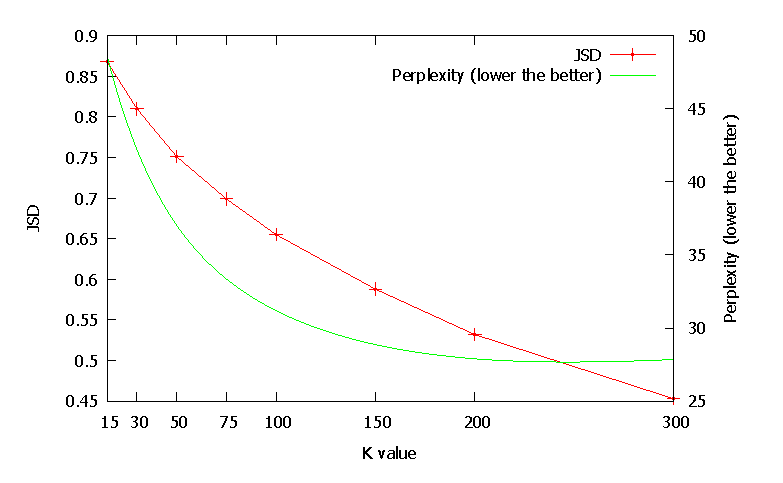
\includegraphics{k}
\caption{不同的\textit{K}值对应的JSD和Perplexity值(URI1模型)}
\label{interest:fig:k}
\end{figure}

同时考虑到模型的泛化能力和重现能力,$JSD$和$Perplexity$是首要关心的指标。在最终实验中选择了$K = 50$作为模型参数。

表\ref{interest:tab:res}展示了所有模型在三个不同数据集上的表现情况。

\begin{table}
\centering
\caption{LDA和URI模型的表现}
\label{interest:tab:res}
\begin{tabular}{|c|c|r|r|} \hline
数据集 & 模型名称 & JSD & Perplexity\\ \hline
\multirow{5}{*}{D0} & LDA0 & 0.040 & 203.805\\ \cline{2-4}
 & LDA1 & 0.211 & 181.824\\ \cline{2-4}
 & LDA2 & 0.211 & 181.824\\ \cline{2-4}
 & URI1 & 0.925 & 98.229\\ \cline{2-4}
 & URI2 & 0.979 & 103.498\\ \cline{2-4}
\hline
\multirow{5}{*}{D1} & LDA0 & 0.079 & 183.021\\ \cline{2-4}
 & LDA1 & 0.307 & 89.910\\ \cline{2-4}
 & LDA2 & 0.990 & 69.853\\ \cline{2-4}
 & URI1 & 0.751 & 34.423\\ \cline{2-4}
 & URI2 & 0.981 & 73.668\\ \cline{2-4}
\hline
\multirow{5}{*}{D2} & LDA0 & 0.064 & 305.282\\ \cline{2-4}
 & LDA1 & 0.247 & 158.881\\ \cline{2-4}
& LDA2 & 0.992 & 64.621\\ \cline{2-4}
 & URI1 & 0.818 & 54.079\\ \cline{2-4}
& URI2 & 0.974 & 121.978\\ \cline{2-4}
\hline\end{tabular}
\end{table}


\section{讨论}
\label{interest:sec:discussion}
本章给出了URI模型及实验结果的讨论,包含实验的结果分析以及给予实验结果的群体行为模式的聚合分析。

\subsection{模型表现分析}
从表\ref{interest:tab:res}中可以看出,总体来说,URI模型的表现显著高于LDA模型。URI2模型发现的隐含``用户兴趣''质量更高,反映出了网站的聚类;而URI1模型能更好的估计每个用户的移动互联网使用行为。这种模型表现可以如下解释:由于URI2中,将地理位置信息作为生成``用户兴趣''时的参数,所以网站在每个``用户兴趣''内的分布与位置无关,而每个``用户兴趣''在每个区域上有一个分布。这就能够更好地将网站聚类,并且将地理位置作为网站类簇的一个特征;另一方面,对于URI1模型,每个网站包含了更多的位置信息,所以其可以更好的估计原始的网站访问分布。由于实验中使用的训练集和测试集时间跨度不大(为连续的时间段),故URI1模型的还原表现更好。

\subsection{群体行为模式聚合分析}
群体行为模式分析,与单个用户的关联较少,与网站的关联较大,如本章中使用URI2模型进行讨论分析。

表\ref{interest:tab:topics}中展示了5个常见的``用户兴趣''及其对应的主题网站。表中还列出了每个用户兴趣的比重,每个用户兴趣中列'出了前5的网站(及其所占比重)作为主题网站。
\begin{table*}
\centering
\caption{URI2模型中的隐含 用户兴趣 层示例}
\label{interest:tab:topics}
\begin{tabular}{|c|r|c|r|c|r|c|r|c|r|} \hline
 \multicolumn{2}{|c|}{兴趣 0} & \multicolumn{2}{|c|}{兴趣 1} & \multicolumn{2}{|c|}{兴趣 2}  \\ \hline
 \multicolumn{2}{|c|}{0.1100} & \multicolumn{2}{|c|}{0.1083} & \multicolumn{2}{|c|}{0.0778}  \\ \hline
weixin.qq.com & 0.8447 & 新浪微博.cn & 0.6761 & z.qq.com & 0.2882\\ \hline
163.com & 0.1424 & sina.cn & 0.3225 & 3g.qq.com & 0.1354 \\ \hline
umeng.com & 0.0059 & 新浪微博.com & 0.0006 & qq.com:8080 & 0.1243\\ \hline
codoon.com & 0.0017 & qik.com & 0.0003 & imtt.qq.com & 0.1115\\ \hline
126.net & 0.0009 & sinaimg.cn & 0.0003 & wap.soso.com & 0.0481\\ \hline

\hline\end{tabular}
\begin{tabular}{|c|r|c|r|} \hline
 \multicolumn{2}{|c|}{兴趣 3} & \multicolumn{2}{|c|}{兴趣 4} \\ \hline
 \multicolumn{2}{|c|}{0.0712} & \multicolumn{2}{|c|}{0.0668} \\ \hline
ucweb.com & 0.3402 & 人人网.com & 0.7282\\ \hline
m.baidu.com & 0.2633 & sina.com.cn & 0.1551\\ \hline
uc.cn & 0.1180 & mafengwo.cn & 0.0599\\ \hline
ucweb.com:80 & 0.0289 & vlingo.com & 0.0212\\ \hline
wap.baidu.com & 0.0253 & emoney.cn & 0.0081\\ \hline

\hline\end{tabular}
\end{table*}

从表中可以看出, 每个``用户兴趣''的主题网站比较集中。兴趣 0 主要是关于\textit{微信},这一当前国内最热门的移动社交应用。这一兴趣同样包含\textit{网易}所提供的门户以及邮箱服务,这说明\textit{微信}用户和\textit{网易}用户的重合度相对更高。兴趣 1 主要包含\textit{微博}这一国内最热门的微博服务。兴趣 2 主要包括\textit{QQ},以及\textit{腾讯}的搜索引擎服务\textit{SOSO}。兴趣 2 的集中性并不十分明显,这是由于\textit{腾讯}提供的服务种类很多,而且他们之间的用户重合度很高。之所以\textit{微信}没有和腾讯其他服务被归到一个兴趣中,是因为\textit{微信}有相对独立的生态系统,与其他腾讯服务的整合度并不太高,而且微信所占的移动互联网使用太高,所以被单独分到一个兴趣之中。兴趣 3 主要包含\textit{百度}以及\textit{UC},这也说明百度的移动客户端并不十分强势,移动流量主要来源于手机浏览器。兴趣 4 主要是关于\textit{人人网},这是一个当前国内(特别是学生中)较为流行的社交网站。

可以看出,``用户兴趣''具有较高的内聚度,能够很好地反映出用户的移动互联网使用行为模式。

经过地理区域发现过程后,数据集中共有265个地理区域。``用户兴趣''在地理区域上的分布$\Psi$计算方式如下:
\[
\psi_{r,z} = \frac{\sum_u{m_{u,r,z}} + \alpha_z}{\sum_{z'}{(\sum_u{m_{u,r,z'}} + \alpha_{z'})}}
\]
其中$m_{u,r,z}$的意义见式\ref{interest:equ:theta2}。

所有区域在数据集上的真实分布记为$\mathbf{ql}$。作为案例研究,表\ref{interest:tab:locs}中展示了两个高热度区域内的主要``用户兴趣''类型。类似表\ref{interest:tab:topics},展示了区域及其频度,以及其排名前五的``用户兴趣''的ID、内容(总结自其主题网站)和在此区域内的频度。

\begin{table}
\centering
\caption{两个示例区域内的 用户兴趣 分布}
\label{interest:tab:locs}
\begin{tabular}{|c|c|c|r|c|c|r|} \hline
 \multicolumn{3}{|c|}{区域 58} & \multicolumn{3}{|c|}{ 区域 0} \\ \hline
 \multicolumn{3}{|c|}{0.0210} & \multicolumn{3}{|c|}{  0.0178} \\ \hline
1 & 新浪微博 & 0.1542 & 0 & 微信 & 0.0971\\ \hline
 0 & 微信 & 0.1120 & 5 & 人人网 & 0.0957\\ \hline
 8 & Apple & 0.0863 & 1 & 新浪微博 & 0.0908\\ \hline
 3 & QQ门户 & 0.0727 & 4 & UC \& Baidu & 0.0844\\ \hline
 5 & 人人网 & 0.0619 & 2 & QQ(腾讯) & 0.0837\\ 
\hline\end{tabular}
\end{table}

区域 58 是一个商业区,该区域内的活跃用户为白领上班族;区域 0 是一个学校区域,该区域内有若干高校,活跃用户主要是高校学生。从表\ref{interest:tab:locs}可以清楚地看到这两个区域在兴趣分布上的区别:在区域 58 中,新浪微博的比重显著高于区域 0,这表明新浪微博在白领中的流行度更高;相反,\textit{人人网}在区域 0 中的比重更高,这说明该服务在高校学生中更为流行。这些发现与根据实际情况的猜想是一致的。

这两个区域的另一个区别在于\textit{苹果公司}网站的比重。这些网站在区域 58 内排名第3,而在区域 0 内却没有排进前5。这说明苹果设备在中国的白领之中市场占有率要普遍高于学生。由于iPhone等苹果设备在中国属于近似奢侈品,价格昂贵,所以其在白领中的受欢迎度更高,白领的购买能力也更强,这一结论也和实际情况比较一致。

\section{本章小结}
\label{interest:sec:conclusion}
本章提出了基于运营商数据进行用户移动互联网上网行为分析的方法。提出了一个根据地点的移动互联网流量来将其划分为地理功能区域的聚类方法;提出了基于概率话题模型的方法,来从移动互联网使用记录中,联系地理区域信息,解析出隐含的``用户兴趣''层。共提出了两个话题模型,并分别将其应用于北京地区的真实运营商数据集,其中覆盖了超过三百万的用户。实验结果表明,模型具有较好的有效性和还原(预测)能力。模型输出了有意义的和用户行为模式。根据模型输出进行了城市级别的聚合用户行为模式的分析,并讨论了不同地理功能区域之间的对比差异。


\chapter{移动用户行为分析平台}
\label{cha:system}

\section{系统概述}
\label{system:sec:intro}
移动环境下的用户行为数据,具有数据量巨大,数据种类繁多,来源多种多样等特点。如何将大量的异构数据进行有效的整合和高校的处理、挖掘,是在移动环境下进行用户行为分析所面临的重要挑战。本章描述的\textbf{移动用户行为分析平台(Mobile Data Analysis Platform,MDAP)},是一个集数据收集、存储、计算和展示为一体的全面的云计算数据挖掘平台。

本平台可分为底层数据存储、统一化的数据集操控API、REST API、可制定数据挖掘模块、数据展示和可视化模块等部分组成。平台的组织架构参见图\ref{mdap:fig:architecture}。

\begin{figure}[htbp]
  \centering
    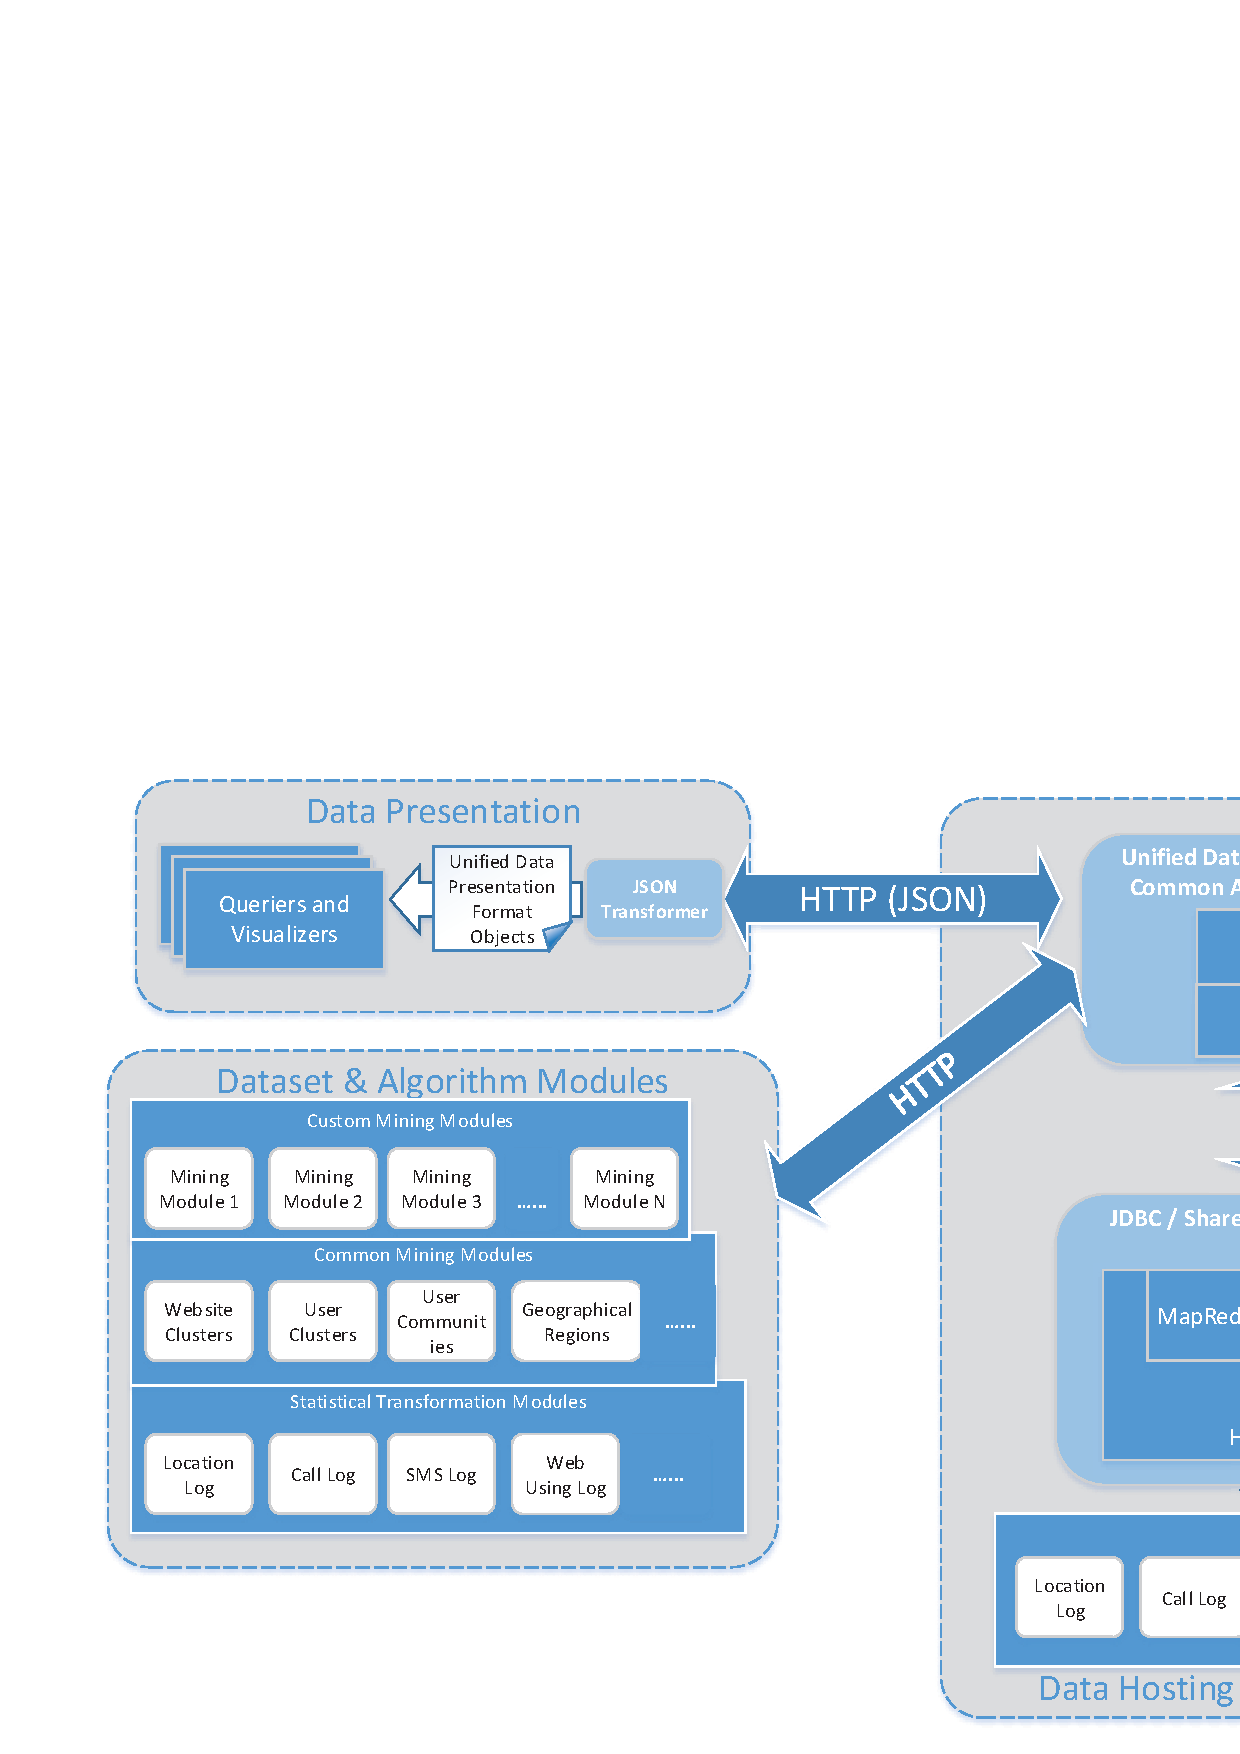
\includegraphics[width=15cm]{mdap}
  \caption{MDAP组织架构图}
  \label{mdap:fig:architecture}
\end{figure}

平台主要提供表格式数据集的添加、访问、增加和删除。在数据的来源方面,平台支持流式的数据输入,可以从移动运营商处通过文件复制或访问数据接口等方式导入,也可由手机客户端通过访问API来写入。平台的手机客户端应用,可以使用不同策略采集多种手机传感器的数据,以及通讯数据和其他手机使用数据。关于手机端采集系统的实现详见第\ref{system:sec:collect}章。

在数据的存储方面,平台底层支持多种异构的数据存储方式,包括Hadoop/HDFS,Hive,SQL关系数据库,以及文本文件等等。数据的存储的运算是否为并行化取决于其低层的的数据存储实现方式。不同的数据存储实现方式通过统一的编程API提供数据操控服务,从而屏蔽了底层实现的异构性,使平台的使用者(数据挖掘研究人员和数据分析师)能够不必关系底层数据存储实现方式,而专注于数据和对数据的分析挖掘。

数据的访问方面,对于挖掘中使用率最高的表格型数据,平台规定了一整套抽象的统一接口,包括数据集元数据的表示方式,数据的查询接口、返回格式和遍历方法,以及数据的写入方法等。关于编程接口的详细描述参见第\ref{system:sec:javaapi}章。同时,平台还提供标准的REST API,给开发者和可视化人员提供远程调用的接口。关于REST接口的详细描述见第\ref{system:sec:restapi}章。

在数据展示方面,不同类型的数据集携带了不同的语义信息(如地理位置、时间序列数据、统计数据等),根据数据集的语义信息可以知道其适合使用哪种形式的图表予以可视化。平台的数据可视化模块,可以根据数据集语义信息API中获取的语义信息对数据集进行通用而又有针对性的可视化展示。有关可视化系统详见第\ref{system:sec:vis}章。



\section{手机端数据采集系统}
\label{system:sec:collect}

手机端产生的传感器数据、通讯数据及手机使用数据等,对用户个体的行为分析十分重要。手机端的数据采集采用手机应用的方式,采集多种不同的手机产生的数据,经过简单的处理转换,而后自动上传到平台中供集中存储和分析。

目前的手机端数据采集应用运行于Android平台。由于手机上的传感器类型及其他类型数据在不同平台上都类似,所以此应用也可以很简单地扩展到其他平台。

\subsection{Android平台传感器概述}
\label{system:sec:AndroidPlatformSensors}

\textbf{Android} \footnote{\url{http://www.android.com/}} 是一个应用于移动设备(手机,平板电脑等)等基于Linux的操作系统\footnote{\url{http://en.wikipedia.org/wiki/Android_(operating_system)}}。
Android包含一个基于Linux的定制内核,以及一个针对移动环境优化过的虚拟运行时环境,称为Dalvik。Android上运行的应用通常由Java语言编写,而后便以为Dalvik的dex-code,而后运行于Dalvik平台。从2007年项目开始至今,Android已经成长为世界上使用最为广泛的智能手机操作系统。 

Android内置支持多种传感器设备。目前,版本号16的Android API描述了11种传感器类型\footnote{\url{http://developer.android.com/reference/android/hardware/Sensor.html}},新的传感器类型还在不断加入中。Android设备方面,声音传感器(麦克风),位置感知功能(通过GPS、WIFI等)以及加速度传感器已几乎成为Android手机的标配。然而,由于采用Android系统的设备种类繁多,并不能保证某一种类的传感器一定会存在于某一台设备上。本系统中采集的传感器数据类型同时考虑了其在不同设备上的可用性以及对用户行为建模的作用。

Android使用广播-接受模式(broadcaster-receiver pattern)来管理传感器。当某一应用需要使用传感器时,首先要向系统注册为该传感器的接收者,与此同时,指定一个接收传感器数据的敏感程度(用以控制频率)。而后,每当传感器的感知数值发生变化(由所设置的敏感程度控制)\cite{sensorevent}。

\begin{itemize}
  \item \textbf{加速度传感器.} Android系统的加速度传感器数据的计算是通过测量传感器本身的受力实现的,其中也包含重力。根据Android系统的三轴定位系统,加速度传感器的读书包含三部分:X轴位水平向右方向,Y轴为垂直向上,Z轴垂直于屏幕向外\cite{sensorevent}。将$t$时刻的的加速度传感器数值即为$(x^{(t)}, y^{(t)}, z^{(t)})$。
  
  加速度传感器可能是Android设备商配备率最高的传感器,而且其能量消耗也较低。加速度传感器数据可以用于探测用户的物理移动情况,这在行为建模上十分重要。
  基于以上原因,加速度传感器在所有传感器数据中处于核心地位。

  \item \textbf{声音传感器.} 严格来说,声音传感器并不属于Android系统的传感器类型。然而,每一部手机都配备有麦克风,可以用来感知用户的声音以及背景声音的强弱。在心境建模方面,环境声音的状态能用影响到用户的心境状态,而用户的声音也能够反映到其心境状态。
  \item \textbf{地理位置.} 地理位置和用户行为也有着紧密的联系,可以作为用户行为的一个重要的上下文信息。Android提供了两种地理位置信息:粗略位置服务和精确位置服务。地理位置可以通过GPS,WiFi以及移动蜂窝网络来获得。由GPS提供的精确位置能够达到3米以内的精度;不使用GPS的定位能够达到数十米的精度,但对于用户行为建模的楼宇级别的定位,这一精度也在可以接受的范围之内。
  \item \textbf{光线传感器.} 环境光线传感器一般用来自动调整屏幕的亮度,控制键盘背景灯等等能。背景光线情况能够反映用户所处的环境,影响到用户的行为。同时,环境光线还能够用来判定手机所处的位置(在衣服口袋里,桌上等)。
\end{itemize}

\subsection{应用实现}
\label{system:sec:ApplicationImplementation}

收集数据手机应用包含如下的数据收集组件:传感器数据收集;通讯数据收集;其他信息收集(如用户情绪自报告)。 

应用的工作流程如下。传感器数据的收集随着应用的启动而开始。对不同类型的传感器数据采用不同的策略记录下来(后文详细描述),收集的传感器数据暂时以文本文件的形式存储于手机内。(Android系统内置有SQLite数据库支持,但其在大量数据的顺序读写上的效率远低于使用纯文本文件,故此处未予采用)。
%
通讯数据的收集发生在每次数据上传行为前,从Android系统的系统日志中获得。通讯信息获取模块从手机中读取短信和通话记录信息,将其中的目标号码,时间以及长度信息存储于手机文本文件中。这些数据可以用来作为通讯频率统计数据来源,也可以作为建立社交网络的数据源。
%
其他信息收集为面向某一特定挖掘任务所需要收集的特殊类型的信息,如心境评估问题中需要的用户心境自报告。心境自报告模块包含一个允许用户报告其心境的图形界面。应用的使用者每天至少一次,每次以三个维度(每个维度有5个离散级别)报告其心境状态。根据应用的设置,每晚十点钟用户情绪报告页面会自动弹出,但用户也可在任何时间通过菜单调出报告界面。此类其他信息同样被以文本文件的形式存储与手机中。

每天手机的数据会在当日末尾上传到平台上。首先在本地将存有传感器数据,通讯数据以及其他数据的文本文件进行压缩,而后在手机有可用的数据连接(移动网络或WiFi,用户可设置)的时候自动上传。

除了基本的数据格式转换外,所有的原始数据都被上传到云端,其余的处理和挖掘工作全部在云端完成。用户可以通过应用获取平台提供的挖掘结果,应用也可以调用平台的数据可视化接口向用户展示统计和挖掘的结果。

图\ref{system:fig:interface}展示了用于心境评估中的应用界面截图。该界面中显示了计算得到的用户行为特征。界面底部给出的心境的评估结果。

\begin{figure}[htbp]
  \centering
    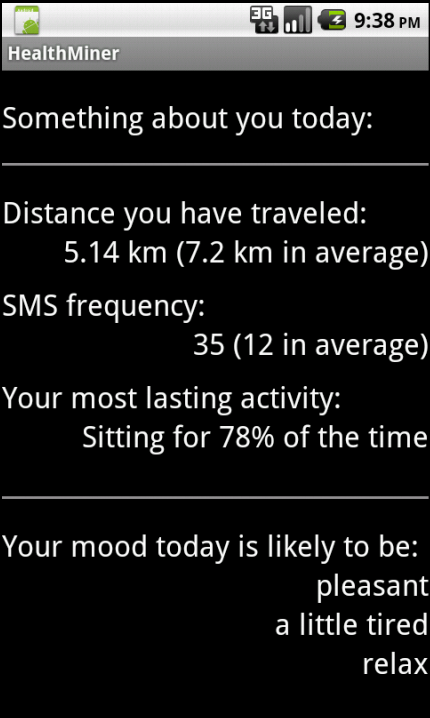
\includegraphics[width=215bp,natwidth=430bp,natheight=718bp]{interface.png}
  \caption{手机端数据展示界面(包括心境)}
  \label{system:fig:interface}
\end{figure}

\subsection{传感器管理策略}
\label{system:sec:SensorManagementStrategy}

手机传感器通常有较高的能耗,高强度地使用手机传感器将会显著地影响手机的电池寿命。在本应用中,针对不同的传感器,使用了不同的生命周期管理方法,从而达到了适应数据采集需要和降低能耗之间的平衡。

对能耗影响最大的两个传感器类型是加速度传感器和定位传感器。

加速度传感器在Android手机上配备最为广泛,其能耗功率也比较低,我们在平台中将加速度传感器数据作为一直需要采集的数据,用来进行用户的姿态检测,动作检测等(示例详见第\ref{mood:sec:ProblemAndFeatureDefinition}章)。然而,虽然加速度传感器的功率相对较低,但由于其数据需求的频率比较高,因此对加速度传感器的管理对最终能耗有较大影响。
% 
当应用接收到加速度传感器数据时,首先将其和之前的读数进行比较。如果新值与原值间的差别不大,认为手机状态没有发生显著变化,则新值不会保存,而且会适当降低数据采样的频率。只有两个值之间差别较大时,说明手机的物理运动状态发生了显著改变(如:被用户用手拿起),才会记录新的加速度值。基于实验观察,最终确定,只有三个轴上的任何一个的读书变化0.5m/s$^2$时才视为显著变化。
  
另一个高耗能的传感数据类型为地理位置。地理位置通常通过GPS或WiFi等渠道获得,这两种方式能耗都比较大。参考Cui等\cite{jianc}的做法,本应用将加速度传感器数据和地理位置相结合,设计了一个自适应的地理位置感知方法。
具体地,在预先设置的时间片$T$内,用加速度传感器的读数粗略地估算地理位置的变化。如果算出的地理位置变化并不明显,意味着设备处于一个相对稳定的状态,这时并不激活GPS或WiFi等位置传感器,而是将上次测得的位置作为当前的位置。为消除累积误差,同时要保证位置传感器在每$T_0$时间段内至少要启动一次。这个策略能够较为精确地感知地理位置,同时显著降低了传感器能耗。


\section{并行化数据分析平台}
\label{system:sec:mdap}
\subsection{平台编程接口的设计与实现}
\label{system:sec:javaapi}
在平台中,所有对底层数据的操作被一套抽象的API所封装,对数据的一切操作都需要通过API调用来实现。API采用Java编程语言,包含了数据集元数据管理,数据查询和访问,数据操纵,数据集语义信息管理等功能。整套API框架中的顶层接口规范见图\ref{system:fig:javaapi}

\begin{figure}[htbp]
  \centering
    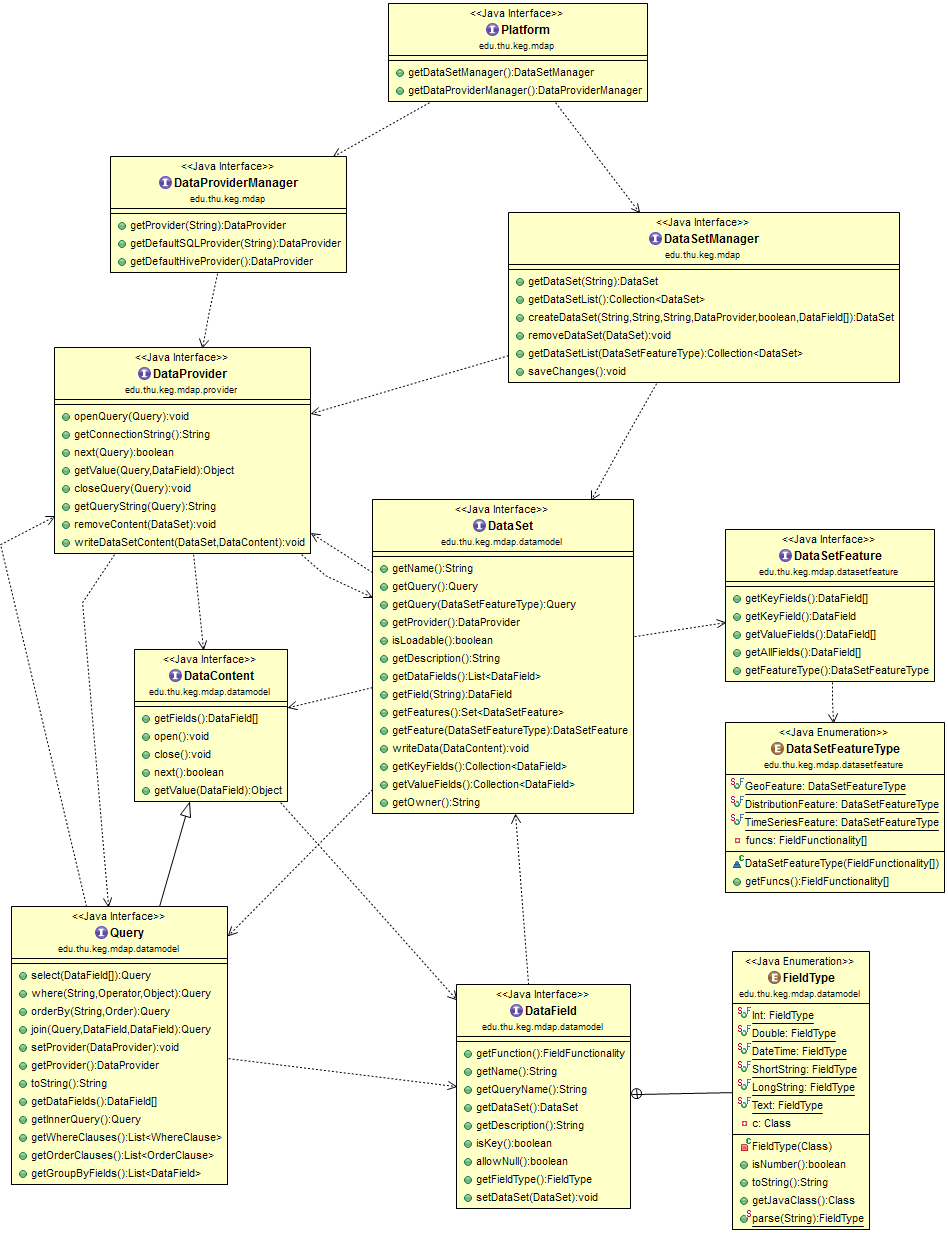
\includegraphics[width=15cm]{api.png}
  \caption{MDAP顶层编程接口规范}
  \label{system:fig:javaapi}
\end{figure}

\textbf{数据集元数据管理.} 
\textbf{数据集}是本平台中管理数据的基本概念。每个数据集描述了移动环境下的一种格式化数据,原始数据集一般来源于设备产生的格式化记录(如手机传感器数据记录、运营商网络设备记录等),数据集也可由其他数据集经过处理得到。另外,格式化的挖掘结果也是一种数据集。数据集的结构类似关系型数据库中的关系表,其元数据中包含若干\textbf{数据列},描述了其中存储的数据的格式。数据集的其他元信息还包括数据集名称,数据集描述,数据集对应的存储提供者等信息。描述数据集元数据的数据对象(Data Obejct,DO)接口 \texttt{DataSet} 见表\ref{system:fig:dataset}。

\begin{table}[htbp]
  \centering 
   \caption{\texttt{DataSet}接口规范}
    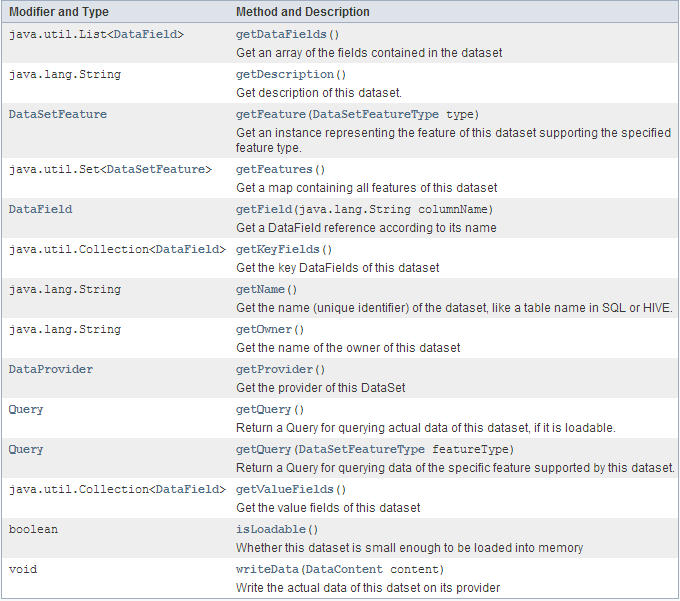
\includegraphics[width=15cm]{dataset.png}
  \label{system:fig:dataset}
\end{table}

数据集的管理通过数据访问对象(Data Access Object,DAO):\texttt{DataSetManager} 来实现。所有数据集的元数据信息以XML形式持久化存储,\texttt{DataSetManager} 封装了数据集新增、查找、更新、保存等多种操作,是获取数据集元数据的唯一途径。

数据列用来描述数据集格式,代表表格型数据中的一列。数据列可能数据某一数据集,也可能在查询中动态生成。数据列的元数据包括数据列名称、类型、语义类型、描述、是否为主键、列值是否有序、以及其所属的数据集等。

\textbf{数据集语义信息管理.} 
为了满足可视化等需要,平台提供了数据集语义信息管理的API。语义信息分为两个层面:数据列语义信息和数据集语义信息。

数据列的语义信息通过记录数据列的语义类型来实现,平台中规定了若干种移动环境下常见的语义类型,见表\ref{system:tab:columnTypes}。根据数据列的语义类型,可将数据列分为两类。一类为属性列,即该列的值代表了观察此数据集的一个维度,可以根据这一列对数据集进行分组统计等进一步分析处理;另一类为实时列,也即值列。这一类的列通常为统计数值或其他数值,可作为进一步统计的目标列,以及用来可视化的数值对象。

\begin{table}
\centering
\caption{数据列的语义类型表}
\label{system:tab:columnTypes}
\begin{tabular}{|c|c|l|} \hline
名称 & 类型 & 描述\\ \hline
纬度 & 属性列 & 地理位置中的纬度\\ \hline
经度 & 属性列 & 地理位置中的经度\\ \hline
编号 & 属性列 & 记录的唯一编号\\ \hline
时间戳 & 属性列 & 记录的时间属性\\ \hline
计数 & 事实列 & 统计数值 \\ \hline
值 & 事实列 & 一般的事实列 \\
\hline\end{tabular}
\end{table}

数据集的语义信息依赖于其包含的所有数据列的语义信息。一个数据集的语义信息主要是其包含哪些属性列的组合。另外,事实列与属性列的搭配关系也属于数据集层面的语义关系。

\textbf{底层数据存储实现的封装.} 

通过规定数据集操作的通用API,屏蔽了底层数据存储实现的细节。在平台中,不同的数据存储实现均作为系统的一个数据提供者(DataProvider)。操作数据集时并不需要关系其后台使用的是哪一个具体的数据提供者。接口 \texttt{DataProvider} 的描述见表\ref{system:fig:dataprovider}。目前已经实现的数据提供者有Hadoop(Hive),JDBC以及纯文本文件。

\begin{table}[htbp]
  \centering 
   \caption{\texttt{DataProvider}接口规范}
    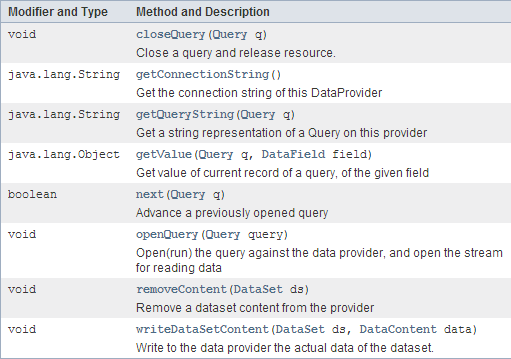
\includegraphics[width=12cm]{provider.png}
  \label{system:fig:dataprovider}
\end{table}

平台提供了数据访问对象 \texttt{DataProviderManager}来对DataProvider进行集中注册和管理。

\textbf{数据查询和访问.} 

为了实现与存储平台的无关性,平台提供了用于查询、遍历和写入数据集数据的通用API。API规定了类 \texttt{DataContent} 作为承载数据内容的对象,通过遍历 \texttt{DataContent}可以得到其每一条记录、每一数据列的值。
获取 \texttt{DataContent}对象,可以通过手动将其他表格型数据转换为 \texttt{DataContent},也可以通过构建 \texttt{Query}对象。\texttt{Query} 类为 \texttt{DataContent}类的子类,负责查询平台上的一个或多个数据集的内容。作为 \texttt{DataContent} 的子类,\texttt{Query} 也可被遍历而得到其数据内容。\texttt{Query} 支持按记录过滤\texttt{where}、按列过滤\texttt{select}、按某些列进行分组统计、排序和内连接等操作。用户可以不关心底层实现,通过调用 \texttt{Query} 对象提供的方法构造各种复杂的查询以满足其需要。各个不同的数据提供者(\texttt{DataProvider})负责将 \texttt{Query} 对象携带的查询信息转换为自身支持的查询格式,并返回查询结果。\texttt{Query} 的描述见表\ref{system:fig:query}

\begin{table}[htbp]
  \centering 
   \caption{\texttt{Query}接口规范}
    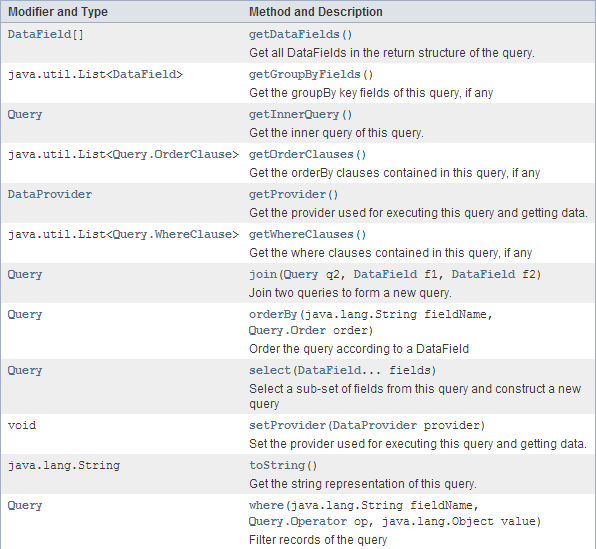
\includegraphics[width=15cm]{query.png}
  \label{system:fig:query}
\end{table}

\subsection{平台远程访问的REST接口设计与实现}
\label{system:sec:restapi}

出于对响应速度、层次的划分的清晰度、扩展度以及开发的便利程度等方面的考虑,平台采用了REST API作为的对外的远程访问接口\cite{pautasso2008restful}。使用REST API,客户端可以利用浏览器的缓存提高用户的响应速度,并且简化了客户端开发和部署的复杂性。

对应与提供后台的数据服务,以及满足平台管理的不同方面的需求,MDAP中的REST API根据功能分为三类:
\begin{itemize}
  \item 数据操作API
  \item 用户管理API
  \item 平台管理API
\end{itemize}

数据操作API对应与平台中队数据集的所有操作,是REST API中最核心的部分。用户可以通过调用数据操作API,设定所需要的参数进行对数据的查询、读取等一系列操作。可以根据数据集的类别、性质、所支持的语义特征等进行针对性的查找。同时针对可视化等前端需求,返回符合要求的多种不同格式的数据集元数据和内容数据。REST API还支持对数据集的增,删,改,查的一系列基本功能,使得使用平台的数据挖掘开发人员和数据分析员可以简单快捷地搭建轻量级的数据探索和展示应用。数据操作API概览见表\ref{system:tab:restapi}。
 
\begin{table}
\centering
\caption{数据操作REST API概览}
\label{system:tab:restapi}
\begin{tabularx}{15cm}{|p{1.3cm}|l|X|} \hline
类别 & URL & 功能 \\ \hline
\multirow{8}{1.3cm}{GET读取} & /mdap/rest/dsg/getdss & 返回所有数据集列表\\ \cline{2-3} 
 & /mdap/rest/dsg/getgeodss & 返回所有包含地理信息数据集列表\\ \cline{2-3}
 & /mdap/rest/dsg/getstadss & 返回所有包含统计信息数据列表\\ \cline{2-3}
 & /mdap/rest/dsg/getds/\textit{datasetname} & 返回数据集\textit{datasetname}的所有信息\\ \cline{2-3}
 & /mdap/rest/dsg/getgeods/\textit{datasetname} & 返回数据集\textit{datasetname}的地理信息\\ \cline{2-3}
 & /mdap/rest/dsg/getstads/\textit{datasetname} & 返回数据集\textit{datasetname}的统计信息\\ \cline{2-3}
 & /mdap/rest/dsg/getstatds/\textit{datasetname} & 返回数据集\textit{datasetname}的时间序列信息\\ \cline{2-3}
 & /mdap/rest/dsg/getdsfds/\textit{datasetname} & 返回数据集\textit{datasetname}的属性信息 \\ \hline
\multirow{3}{1.3cm}{POST创建} & /mdap/rest/dsp/addds/\textit{datasetname} & 添加数据集\textit{datasetname}\\ \cline{2-3}
 & /mdap/rest/dsp/getdsf/\textit{datasetname} & 返回数据集\textit{datasetname}的fieldname列\\ \cline{2-3}
 & /mdap/rest/dsp/getdsres/\textit{datasetname} & 返回数据集\textit{datasetname}的符合fieldname列的值opr特定value值的所有数据 \\ \hline
DELETE删除 & /mdap/rest/dsd/rmds/\textit{datasetname} & 删除数据集\textit{datasetname} \\

\hline\end{tabularx}
\end{table}

用户管理API支持基于用户和角色的访问控制和权限管理。平台提供标准的注册、登陆和基本信息管理的功能,并将用户账户与底层数据平台相联系。同时,为提供基于用户账户的管理和个性化展示,用户管理API还允许每个用户保存、定制自身关注的数据集和可视化结果。

平台管理API在数据管理、用户管理的基础上,提供了更多的平台管理功能。用户可以通过REST API将调用平台SDK的程序包文件验证身份后上传到平台运行,并通过平台管理API查询任务的运行状态。另外,平台上注册的所有数据提供者,支持的语义信息类型等管理数据,也可通过平台管理API查看。

\section{数据可视化模块}
\label{system:sec:vis}

平台利用数据集保存的语义信息,提供了对不同类别的数据集进行有针对性的、可配置的可视化展示。目前,平台支持两大类数据可视化方法:地图可视化和统计数据可视化。含有\emph{维度}、\emph{经度}(参见第\ref{system:sec:javaapi}章)的数据集即可被地图可视化。平台提供灵活的可视化配置,可选择在地图上显示数据集中其他各种不同的附加信息。地图可视化界面样例参见图
\ref{mdap:fig:map}。

\begin{figure}[htbp]
  \centering
    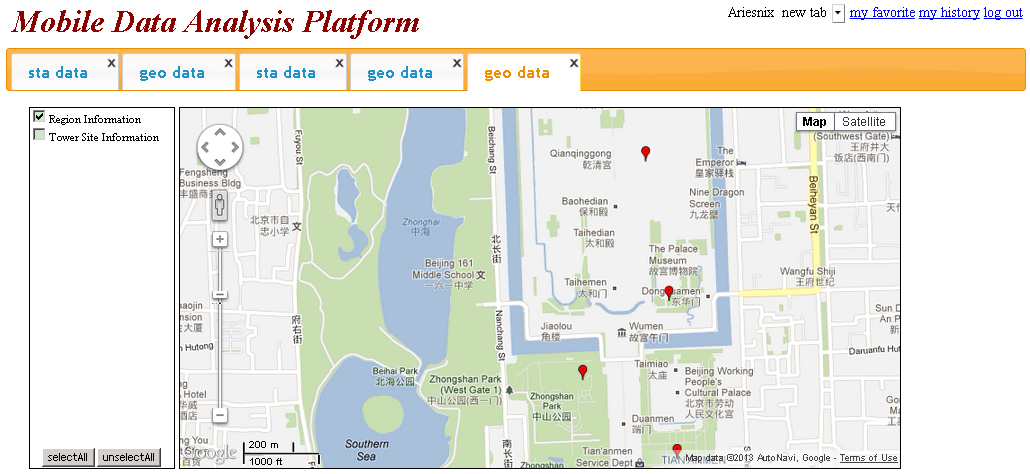
\includegraphics[width=15cm]{geo.png}
  \caption{地图可视化结果样例}
  \label{mdap:fig:map}
\end{figure}
统计可视化则更加灵活。借助数据集的主键域(属性域)和事实域(值域)信息,可灵活使用和配置不同的统计可视化工具,目前支持的有饼图(用以显示比例分布)、折线图(用以显示带时间属性的数据值)、柱状图(对比一个或多个系列的绝对取值大小)等。统计可视化界面样例参见图
\ref{mdap:fig:sta}。


\begin{figure}[htbp]
  \centering
    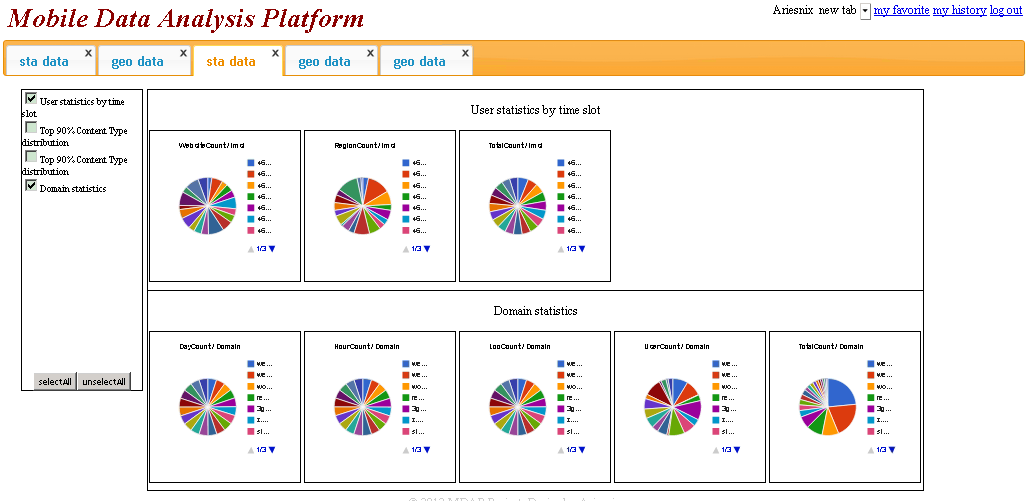
\includegraphics[width=15cm]{sta.png}
  \caption{统计可视化结果样例}
  \label{mdap:fig:sta}
\end{figure}

\section{本章小结}
\label{system:sec:conclusion}

本章展示了用于移动环境下用户行为分析的\textbf{移动用户行为分析平台(Mobile Data Analysis Platform,MDAP)}。首先给出了MDAP的总体架构介绍,包括数据收集模块、数据分析平台和数据展示模块。而后详细描述了Android移动平台上的数据收集应用。包括Android平台传感器介绍,应用收集的数据类型、收集方式,以及传感器数据的收集策略和传感器能耗管理策略等。数据分析平台方面,详细描述了以数据集为主要操作对象的编程接口的设计与实现,通过规定标准的数据操控编程接口实现了对底层数据存储细节的屏蔽,以及不同来源、不同存储方式的数据集的统一操作和继集成,同时还给出了平台REST API的详细描述。最后,描述了系统支持图形化数据浏览和数据可视化的模块,实现了对数据集的通用且有针对性的展示和可视化。
\chapter{总结及未来工作}
\label{cha:conclusion}

\section{论文总结}
利用海量的互联网记录数据和移动设备使用记录数据进行用户行为的分析和挖掘,是互联网及数据挖掘领域的重要课题,在面向个人和群体的多种服务上都有重要应用。本文利用移动环境下在设备端和运营商网络端产生的海量多种类数据,应用用户行为分析方法,针对个人用户的心境评估,以及群体用户的上网行为模式分析等问题提出了解决方法,并设计实现了完整的移动数据挖掘平台。

基于手机数据的个人心境评估方法中,首先给出了心境及心境评估问题的现状描述,并给出了运用移动环境下用户行为分析方法进行心境评估问题的上下文的形式化定义和描述;而后根据手机端可收集的用户行为相关的数据类型,定义了基于手机感知数据的用户行为特征,然后通过对实验数据的观察分析,结合心理学背景知识,使用概率因子图模型将社交关系、历史心境关系和用户行为特征统一建模,来评估用户心境。只使用历史心境和简单用户行为特征的模型,实验结果的评估精度达到了50\%;使用历史心境、所有用户行为特征和社交关系的完整模型的评估精度达到了70\%。

基于移动运营商数据的用户上网行为分析中,首先给出了所用的数据集规模、特征等概况描述,而后提出了基于用户与地理位置相关的上网行为,对地理位置进行功能区域划分的方法,并提出了将用户访问的主机地址聚类为网站的方法。在概率话题模型中,将地理功能区域、网站、用户等数据综合考虑,得出隐含的``用户兴趣''(网站类簇),从而对用户的移动互联网上网行为模式进行分析。实验中使用不同的评价指标计算了模型可靠度和还原(预测能力),结果表明,考虑到地理位置等附加因素的模型在各方面均有良好的表现,模型输出中发现了有意义的群体用户上网行为模式。

移动数据分析平台,包含了数据存储、处理、挖掘、可视化等完整的数据分析流程,实现了并行化的海量多来源异构数据的集成和挖掘。首先描述了平台定义的统一的Java语言编程接口,完整地支持对结构化和非结构化数据的查询、读取、写入等所有基本操作,实现了对异构的底层数据存储方式的封装。而后描述了平台的REST API,通过该标准接口实现了对远程调用的支持。而后描述了平台的数据可视化模块,支持针对数据集特征的不同,使用不同的可视化方法(地图可视化;统计可视化如饼图、折线图、柱状图等等)对其进行可配置的数据可视化。最后展示了平台的图形化管理界面。

\section{未来工作}

随着移动计算设备和移动互联网的飞速发展,移动环境下的用户行为分析定将持续成为热门的研究课题。下一步研究中可以考虑更多更丰富的用户行为数据,并且将用户行为分析方法应用到其他与行为相关的建模问题中。

应用手机数据进行心境评估方面,可以考虑更多的上下文信息,包括天气,以及用户所到过位置发生过的公共事件等。 在手机感知数据的处理方面,可以用不同来源的传感器数据定义整合的用户行为特征,从而改进模型的表现。

基于运营商数据进行用户上网行为分析方面,可以将用户间的社交关系考虑进模型。移动互联网中的上网行为可能通过社交网络进行传播,因此根据社交关系(通讯记录,同地同现等)来建立社交网络可以给每个用户更丰富的的上下文信息,从而改善模型的精确度。

移动数据分析平台方面,可以拓展平台支持的底层数据存储方式,同时支持更多的数据可视化方法和格式。同时在跨数据源的数据集成等方面从平台层面予以更多的支持。




%%% 其它部分
\backmatter

% 本科生要这几个索引,研究生不要。选择性留下。
% \makeatletter
% \ifthu@bachelor
%   % 插图索引
%   \listoffigures
%   % 表格索引
%   \listoftables
%   % 公式索引
%   \listofequations
% \fi
% \makeatother


% 参考文献
\bibliographystyle{thubib}
\bibliography{ref/refs}

% 致谢

%%% Local Variables:
%%% mode: latex
%%% TeX-master: "../main"
%%% End:

\begin{ack}

  感谢感谢感谢
  % 衷心感谢导师许斌教授对我在科研和生活上的指导。三年的硕士研究生学习中,能作为许斌老师的学生,令我倍感荣幸。这段宝贵的经历必将使我终身获益。

  % 承蒙李娟子教授和唐杰福教授对我热心指导和帮助,不胜感激。感谢张鹏老师对我在很多实践性问题上的指导。他们的指导和影响使我受益匪浅。

  % 感谢实验室全体同学。三年的研究生生活,实验室活跃向上的治学氛围给了我莫大的帮助。

  % 感谢家人在学习生活的各方各面给我的关心和支持。

  % 感谢我的妻子朱润,在攻读硕士学位的道路上与我携手并肩,给予我巨大的支持和帮助。你是我最宝贵的财富。
\end{ack}


% 附录
% \begin{appendix}
% %%% Local Variables: 
%%% mode: latex
%%% TeX-master: "../main"
%%% End: 

\chapter{外文资料原文}
\label{cha:engorg}
As one of the most widely used techniques in operations research, {\em
  mathematical programming} is defined as a means of maximizing a quantity known
as {\em objective function}, subject to a set of constraints represented by
equations and inequalities. Some known subtopics of mathematical programming are
linear programming, nonlinear programming, multiobjective programming, goal
programming, dynamic programming, and multilevel programming$^{[1]}$.

It is impossible to cover in a single chapter every concept of mathematical
programming. This chapter introduces only the basic concepts and techniques of
mathematical programming such that readers gain an understanding of them
throughout the book$^{[2,3]}$.


\section{Single-Objective Programming}
The general form of single-objective programming (SOP) is written
as follows,
\begin{equation}\tag*{(123)} % 如果附录中的公式不想让它出现在公式索引中,那就请
                             % 用 \tag*{xxxx}
\left\{\begin{array}{l}
\max \,\,f(x)\\[0.1 cm]
\mbox{subject to:} \\ [0.1 cm]
\qquad g_j(x)\le 0,\quad j=1,2,\cdots,p
\end{array}\right.
\end{equation}
which maximizes a real-valued function $f$ of
$x=(x_1,x_2,\cdots,x_n)$ subject to a set of constraints.

\newtheorem{mpdef}{Definition}[chapter]
\begin{mpdef}
In SOP, we call $x$ a decision vector, and
$x_1,x_2,\cdots,x_n$ decision variables. The function
$f$ is called the objective function. The set
\begin{equation}\tag*{(456)} % 这里同理,其它不再一一指定。
S=\left\{x\in\Re^n\bigm|g_j(x)\le 0,\,j=1,2,\cdots,p\right\}
\end{equation}
is called the feasible set. An element $x$ in $S$ is called a
feasible solution.
\end{mpdef}

\newtheorem{mpdefop}[mpdef]{Definition}
\begin{mpdefop}
A feasible solution $x^*$ is called the optimal
solution of SOP if and only if
\begin{equation}
f(x^*)\ge f(x)
\end{equation}
for any feasible solution $x$.
\end{mpdefop}

One of the outstanding contributions to mathematical programming was known as
the Kuhn-Tucker conditions\ref{eq:ktc}. In order to introduce them, let us give
some definitions. An inequality constraint $g_j(x)\le 0$ is said to be active at
a point $x^*$ if $g_j(x^*)=0$. A point $x^*$ satisfying $g_j(x^*)\le 0$ is said
to be regular if the gradient vectors $\nabla g_j(x)$ of all active constraints
are linearly independent.

Let $x^*$ be a regular point of the constraints of SOP and assume that all the
functions $f(x)$ and $g_j(x),j=1,2,\cdots,p$ are differentiable. If $x^*$ is a
local optimal solution, then there exist Lagrange multipliers
$\lambda_j,j=1,2,\cdots,p$ such that the following Kuhn-Tucker conditions hold,
\begin{equation}
\label{eq:ktc}
\left\{\begin{array}{l}
    \nabla f(x^*)-\sum\limits_{j=1}^p\lambda_j\nabla g_j(x^*)=0\\[0.3cm]
    \lambda_jg_j(x^*)=0,\quad j=1,2,\cdots,p\\[0.2cm]
    \lambda_j\ge 0,\quad j=1,2,\cdots,p.
\end{array}\right.
\end{equation}
If all the functions $f(x)$ and $g_j(x),j=1,2,\cdots,p$ are convex and
differentiable, and the point $x^*$ satisfies the Kuhn-Tucker conditions
(\ref{eq:ktc}), then it has been proved that the point $x^*$ is a global optimal
solution of SOP.

\subsection{Linear Programming} 
\label{sec:lp}

If the functions $f(x),g_j(x),j=1,2,\cdots,p$ are all linear, then SOP is called
a {\em linear programming}.

The feasible set of linear is always convex. A point $x$ is called an extreme
point of convex set $S$ if $x\in S$ and $x$ cannot be expressed as a convex
combination of two points in $S$. It has been shown that the optimal solution to
linear programming corresponds to an extreme point of its feasible set provided
that the feasible set $S$ is bounded. This fact is the basis of the {\em simplex
  algorithm} which was developed by Dantzig as a very efficient method for
solving linear programming.
\begin{table}[ht]
\centering
  \centering
  \caption*{Table~1\hskip1em This is an example for manually numbered table, which
    would not appear in the list of tables}
  \label{tab:badtabular2}
  \begin{tabular}[c]{|c|m{0.8in}|c|c|c|c|c|}\hline
    \multicolumn{2}{|c|}{Network Topology} & \# of nodes & 
    \multicolumn{3}{c|}{\# of clients} & Server \\\hline
    GT-ITM & Waxman Transit-Stub & 600 &
    \multirow{2}{2em}{2\%}& 
    \multirow{2}{2em}{10\%}& 
    \multirow{2}{2em}{50\%}& 
    \multirow{2}{1.2in}{Max. Connectivity}\\\cline{1-3}
    \multicolumn{2}{|c|}{Inet-2.1} & 6000 & & & &\\\hline
    \multirow{2}{1in}{Xue} & Rui  & Ni &\multicolumn{4}{c|}{\multirow{2}*{\thuthesis}}\\\cline{2-3}
    & \multicolumn{2}{c|}{ABCDEF} &\multicolumn{4}{c|}{} \\\hline
\end{tabular}  
\end{table}

Roughly speaking, the simplex algorithm examines only the extreme points of the
feasible set, rather than all feasible points. At first, the simplex algorithm
selects an extreme point as the initial point. The successive extreme point is
selected so as to improve the objective function value. The procedure is
repeated until no improvement in objective function value can be made. The last
extreme point is the optimal solution.

\subsection{Nonlinear Programming}

If at least one of the functions $f(x),g_j(x),j=1,2,\cdots,p$ is nonlinear, then
SOP is called a {\em nonlinear programming}.

A large number of classical optimization methods have been developed to treat
special-structural nonlinear programming based on the mathematical theory
concerned with analyzing the structure of problems.
\begin{figure}[h]
  \centering
  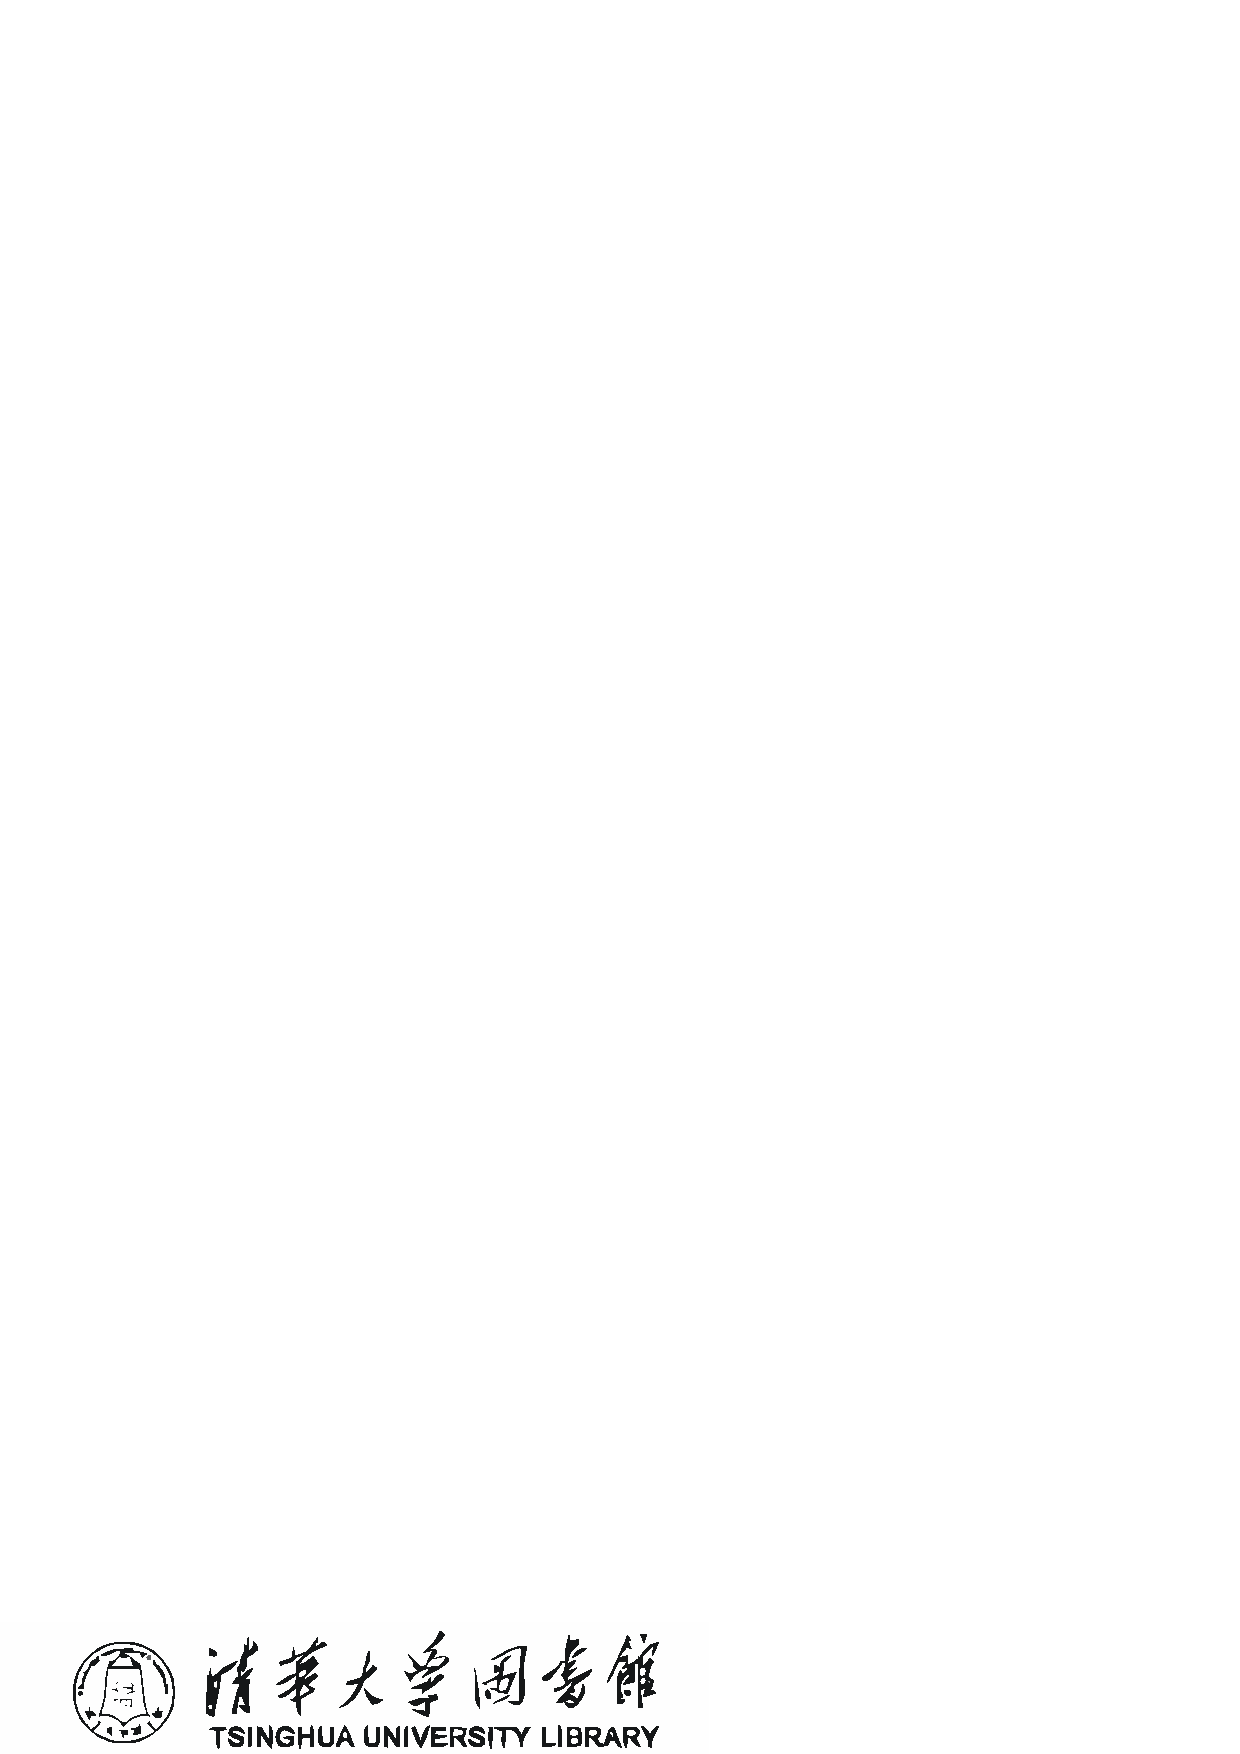
\includegraphics[clip]{thu-lib-logo}
  \caption*{Figure~1\hskip1em This is an example for manually numbered figure,
    which would not appear in the list of figures}
  \label{tab:badfigure2}    
\end{figure}

Now we consider a nonlinear programming which is confronted solely with
maximizing a real-valued function with domain $\Re^n$.  Whether derivatives are
available or not, the usual strategy is first to select a point in $\Re^n$ which
is thought to be the most likely place where the maximum exists. If there is no
information available on which to base such a selection, a point is chosen at
random. From this first point an attempt is made to construct a sequence of
points, each of which yields an improved objective function value over its
predecessor. The next point to be added to the sequence is chosen by analyzing
the behavior of the function at the previous points. This construction continues
until some termination criterion is met. Methods based upon this strategy are
called {\em ascent methods}, which can be classified as {\em direct methods},
{\em gradient methods}, and {\em Hessian methods} according to the information
about the behavior of objective function $f$. Direct methods require only that
the function can be evaluated at each point. Gradient methods require the
evaluation of first derivatives of $f$. Hessian methods require the evaluation
of second derivatives. In fact, there is no superior method for all
problems. The efficiency of a method is very much dependent upon the objective
function.

\subsection{Integer Programming}

{\em Integer programming} is a special mathematical programming in which all of
the variables are assumed to be only integer values. When there are not only
integer variables but also conventional continuous variables, we call it {\em
  mixed integer programming}. If all the variables are assumed either 0 or 1,
then the problem is termed a {\em zero-one programming}. Although integer
programming can be solved by an {\em exhaustive enumeration} theoretically, it
is impractical to solve realistically sized integer programming problems. The
most successful algorithm so far found to solve integer programming is called
the {\em branch-and-bound enumeration} developed by Balas (1965) and Dakin
(1965). The other technique to integer programming is the {\em cutting plane
  method} developed by Gomory (1959).

\hfill\textit{Uncertain Programming\/}\quad(\textsl{BaoDing Liu, 2006.2})

\section*{References}
\noindent{\itshape NOTE: these references are only for demonstration, they are
  not real citations in the original text.}

\begin{enumerate}[{$[$}1{$]$}]
\item Donald E. Knuth. The \TeX book. Addison-Wesley, 1984. ISBN: 0-201-13448-9
\item Paul W. Abrahams, Karl Berry and Kathryn A. Hargreaves. \TeX\ for the
  Impatient. Addison-Wesley, 1990. ISBN: 0-201-51375-7
\item David Salomon. The advanced \TeX book.  New York : Springer, 1995. ISBN:0-387-94556-3
\end{enumerate}

\chapter{外文资料的调研阅读报告或书面翻译}
\section{单目标规划}
北冥有鱼,其名为鲲。鲲之大,不知其几千里也。化而为鸟,其名为鹏。鹏之背,不知其几
千里也。怒而飞,其翼若垂天之云。是鸟也,海运则将徙于南冥。南冥者,天池也。 
\begin{equation}\tag*{(123)}
 p(y|\mathbf{x}) = \frac{p(\mathbf{x},y)}{p(\mathbf{x})}=
\frac{p(\mathbf{x}|y)p(y)}{p(\mathbf{x})}
\end{equation}

吾生也有涯,而知也无涯。以有涯随无涯,殆已!已而为知者,殆而已矣!为善无近名,为
恶无近刑,缘督以为经,可以保身,可以全生,可以养亲,可以尽年。

\subsection{线性规划}
庖丁为文惠君解牛,手之所触,肩之所倚,足之所履,膝之所倚,砉然响然,奏刀騞然,莫
不中音,合于桑林之舞,乃中经首之会。
\begin{table}[ht]
\centering
  \centering
  \caption*{表~1\hskip1em 这是手动编号但不出现在索引中的一个表格例子}
  \label{tab:badtabular3}
  \begin{tabular}[c]{|c|m{0.8in}|c|c|c|c|c|}\hline
    \multicolumn{2}{|c|}{Network Topology} & \# of nodes & 
    \multicolumn{3}{c|}{\# of clients} & Server \\\hline
    GT-ITM & Waxman Transit-Stub & 600 &
    \multirow{2}{2em}{2\%}& 
    \multirow{2}{2em}{10\%}& 
    \multirow{2}{2em}{50\%}& 
    \multirow{2}{1.2in}{Max. Connectivity}\\\cline{1-3}
    \multicolumn{2}{|c|}{Inet-2.1} & 6000 & & & &\\\hline
    \multirow{2}{1in}{Xue} & Rui  & Ni &\multicolumn{4}{c|}{\multirow{2}*{\thuthesis}}\\\cline{2-3}
    & \multicolumn{2}{c|}{ABCDEF} &\multicolumn{4}{c|}{} \\\hline
\end{tabular}  
\end{table}

文惠君曰:“嘻,善哉!技盖至此乎?”庖丁释刀对曰:“臣之所好者道也,进乎技矣。始臣之
解牛之时,所见无非全牛者;三年之后,未尝见全牛也;方今之时,臣以神遇而不以目视,
官知止而神欲行。依乎天理,批大郤,导大窾,因其固然。技经肯綮之未尝,而况大坬乎!
良庖岁更刀,割也;族庖月更刀,折也;今臣之刀十九年矣,所解数千牛矣,而刀刃若新发
于硎。彼节者有间而刀刃者无厚,以无厚入有间,恢恢乎其于游刃必有余地矣。是以十九年
而刀刃若新发于硎。虽然,每至于族,吾见其难为,怵然为戒,视为止,行为迟,动刀甚微,
謋然已解,如土委地。提刀而立,为之而四顾,为之踌躇满志,善刀而藏之。”

文惠君曰:“善哉!吾闻庖丁之言,得养生焉。”


\subsection{非线性规划}
孔子与柳下季为友,柳下季之弟名曰盗跖。盗跖从卒九千人,横行天下,侵暴诸侯。穴室枢
户,驱人牛马,取人妇女。贪得忘亲,不顾父母兄弟,不祭先祖。所过之邑,大国守城,小
国入保,万民苦之。孔子谓柳下季曰:“夫为人父者,必能诏其子;为人兄者,必能教其弟。
若父不能诏其子,兄不能教其弟,则无贵父子兄弟之亲矣。今先生,世之才士也,弟为盗
跖,为天下害,而弗能教也,丘窃为先生羞之。丘请为先生往说之。”
\begin{figure}[h]
  \centering
  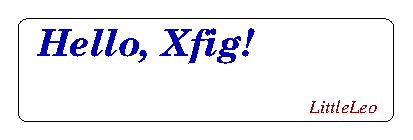
\includegraphics{hello}
  \caption*{图~1\hskip1em 这是手动编号但不出现索引中的图片的例子}
  \label{tab:badfigure3}    
\end{figure}

柳下季曰:“先生言为人父者必能诏其子,为人兄者必能教其弟,若子不听父之诏,弟不受
兄之教,虽今先生之辩,将奈之何哉?且跖之为人也,心如涌泉,意如飘风,强足以距敌,
辩足以饰非。顺其心则喜,逆其心则怒,易辱人以言。先生必无往。”

孔子不听,颜回为驭,子贡为右,往见盗跖。

\subsection{整数规划}
盗跖乃方休卒徒大山之阳,脍人肝而餔之。孔子下车而前,见谒者曰:“鲁人孔丘,闻将军
高义,敬再拜谒者。”谒者入通。盗跖闻之大怒,目如明星,发上指冠,曰:“此夫鲁国之
巧伪人孔丘非邪?为我告之:尔作言造语,妄称文、武,冠枝木之冠,带死牛之胁,多辞缪
说,不耕而食,不织而衣,摇唇鼓舌,擅生是非,以迷天下之主,使天下学士不反其本,妄
作孝弟,而侥幸于封侯富贵者也。子之罪大极重,疾走归!不然,我将以子肝益昼餔之膳。”


\chapter{其它附录}
前面两个附录主要是给本科生做例子。其它附录的内容可以放到这里,当然如果你愿意,可
以把这部分也放到独立的文件中,然后将其 \verb|\input| 到主文件中。
% \end{appendix}

% 个人简历
\begin{resume}

  \resumeitem{个人简历}

  1989 年 5 月 26 日出生于辽宁省盖州市。
  
  2006 年 9 月考入北京工商大学大学计算机科学与技术系,2010 年 7 月本科毕业并获得工学学士学位。
  
  2010 年 9 月通过研究生入学统一考试进入清华大学计算机科学与技术系攻读硕士学位至今。

  \resumeitem{发表的学术论文} % 发表的和录用的合在一起

  \begin{enumerate}[{[}1{]}]
  \item Ma Y, Xu B, Bai Y, et al. Building linked open university data: tsinghua university open data
as a showcase. volume 7185 LNCS, Hangzhou, China, 2012. 385 – 393 (EI 收录,检索号20122515123980)

  \item Ma Y, Xu B, Bai Y, et al. Daily mood assessment based on mobile phone sensing. London,
United kingdom, 2012. 142 – 147. (EI 收录,检索号20122515131481)

  \item Ma Y, Xu B, Bai Y, et al. Infer Daily Mood using Mobile Phone Sensing. Ad Hoc \& Sensor Wireless Networks (已录用,SCI收录)

  \item Yin  Bai, Bin Xu, Yuanchao Ma,  et al.  Will you have a good sleep tonight? sleep quality prediction with mobile phone. The 7th International Conference on Body Area Networks (BodyNets 201 2). Oslo, Norway, September 2012.

  \item Bin  Xu,  Jian  Cui,  Guodong  Sun,  Yuanchao  Ma,  "Demo  Abstract:  Activity-aware  Heart  Sensing  in  Mobile
Healthcare", mHealthSys, in the 9th ACM Conference on Embedded Networked Sensor Systems (SenSys '11)

  \item Ma Y, Xu B, Yuan B, et al. User Behavior Analysis in Mobile Web. 19th ACM SIGKDD Conference on Knowledge Discovery and Data Mining (KDD) (在投)
  \end{enumerate}

  % \resumeitem{研究成果} % 有就写,没有就删除
  % \begin{enumerate}[{[}1{]}]
  % \item 任天令, 杨轶, 朱一平, 等. 硅基铁电微声学传感器畴极化区域控制和电极连接的
  %   方法: 中国, CN1602118A. (中国专利公开号.)
  % \item Ren T L, Yang Y, Zhu Y P, et al. Piezoelectric micro acoustic sensor
  %   based on ferroelectric materials: USA, No.11/215, 102. (美国发明专利申请号.)
  % \end{enumerate}
\end{resume}

\end{document}
